% \iffalse meta-comment
%
% Copyright (C) 2015-2016 by Tibor Tomacs
%
% This file may be distributed and/or modified under the
% conditions of the LaTeX Project Public License, either version 1.2
% of this license or (at your option) any later version.
% The latest version of this license is in:
%
% http://www.latex-project.org/lppl.txt
%
% and version 1.2 or later is part of all distributions of LaTeX
% version 1999/12/01 or later.
%
% \fi
%
% \iffalse
%<*driver>
\ProvidesFile{bookcover.dtx}
\newcommand{\eifiledate}{2016/11/12}
\newcommand{\eifilever}{v2.0}
%</driver>
%<class>\NeedsTeXFormat{LaTeX2e}[1999/12/01]
%<class>\ProvidesClass{bookcover}[2016/11/12 v2.0 class for book covers and dust jackets]
%
%<*driver>
\documentclass{ltxdoc}
\usepackage[utf8]{inputenc}
\usepackage[T1]{fontenc}
\usepackage[paperwidth=210mm,paperheight=295mm,textwidth=160mm,top=25mm,bottom=25mm,outer=25mm]{geometry}
\usepackage[unicode,pdfstartview=FitH,bookmarksnumbered,pdfborder={0 0 0},colorlinks,linktocpage,allcolors=teal]{hyperref}
\usepackage[english]{babel}
\usepackage{xcolor,graphicx,listings,calc,multirow,caption,float,array,pdfpages,fontawesome,tcolorbox,tikz}

\colorlet{command}{blue!80!black}
\colorlet{example}{black}
\colorlet{layer}{purple}
\colorlet{param}{green!50!black}

\lstnewenvironment{examplelst}{\lstset{
    gobble=2,
    belowskip=\bigskipamount,
    basicstyle=\color{example}\small\ttfamily,
    backgroundcolor=\color{black!10},
    columns=fullflexible,
    keepspaces}}{}

\lstnewenvironment{commandlinelst}{\lstset{
    gobble=2,
    basicstyle=\small\ttfamily,
    belowskip=\medskipamount,
    backgroundcolor=\color{white},
    columns=fullflexible,
    keepspaces}}{}

\lstnewenvironment{commandlst}{\lstset{
    literate={<}{{$\langle$}}1{>}{{$\rangle$}}1,
    delim=[is][\color{param}\normalfont\itshape\small]{!}{!},
    gobble=2,
    basicstyle=\color{command}\ttfamily,
    backgroundcolor=\color{white},
    columns=fullflexible,
    keepspaces}}{}

\lstdefinestyle{examplefile}{
    literate={ü}{{\"u}}1{ó}{{\'o}}1{é}{{\'e}}1{á}{{\'a}}1{Á}{{\'A}}1,
    belowskip=\bigskipamount,
    basicstyle=\color{example}\small\ttfamily,
    backgroundcolor=\color{black!10},
    columns=fullflexible,
    keepspaces,
    comment=[l][\ttfamily\color{black!50}]{\%}}

\newcommand{\commandinline}{\lstinline[
    literate={<}{{$\langle$}}1{>}{{$\rangle$}}1,
    delim={[is][\color{param}\normalfont\itshape\small]{!}{!}},
    basicstyle=\color{command}\ttfamily,
    columns=fullflexible,
    keepspaces]}

\flushbottom

\def\meta#1{{\color{param}\normalfont\itshape\small$\langle$#1$\rangle$}}

\usetikzlibrary{shapes}
\def\example{\tikz\draw node[signal,signal from=west,signal to=east,inner sep=2.7pt,left color=command,right color=black,text=white]{\footnotesize\sffamily EXAMPLE};}

\tcbuselibrary{skins}
\newtcolorbox{info}{enhanced jigsaw,frame style={left color=red,right color=black},colback=white,lifted shadow={1mm}{-2mm}{3mm}{0.1mm}{fill=black!50!white,opacity=0.5}}

\def\BookCover{{\def\sfdefault{ugq}\sffamily\bfseries
    \color{gray}\mbox{}\lower.15ex\hbox{[B}ook%
    \color{orange}\lower.15ex\hbox{C}over\lower.15ex\hbox{]}}}

\begin{document}
    \DocInput{./bookcover.dtx}
\end{document}
%</driver>
% \fi
%
% \CheckSum{2556}
%
% \CharacterTable
% {Upper-case \A\B\C\D\E\F\G\H\I\J\K\L\M\N\O\P\Q\R\S\T\U\V\W\X\Y\Z
%     Lower-case \a\b\c\d\e\f\g\h\i\j\k\l\m\n\o\p\q\r\s\t\u\v\w\x\y\z
%     Digits \0\1\2\3\4\5\6\7\8\9
%     Exclamation         \!     Double quote    \"     Hash (number)   \#
%     Dollar              \$     Percent         \%     Ampersand       \&
%     Acute accent        \'     Left paren      \(     Right paren     \)
%     Asterisk            \*     Plus            \+     Comma           \,
%     Minus               \-     Point           \.     Solidus         \/
%     Colon               \:     Semicolon       \;     Less than       \<
%     Equals              \=     Greater than    \>     Question mark   \?
%     Commercial at       \@     Left bracket    \[     Backslash       \\
%     Right bracket       \]     Circumflex      \^     Underscore      \_
%     Grave accent        \`     Left brace      \{     Vertical bar    \|
%     Right brace         \}     Tilde           \~}
%
% \GetFileInfo{bookcover.cls}
%
% \title{{\Huge\BookCover\\[5mm]}
%        Class for book covers and dust jackets\\
%        \textsf{bookcover.cls}\\
%        {\large\eifilever\ (\eifiledate)}}
% \author{Tibor Tómács\\{\normalsize\href{mailto:tomacs.tibor@uni-eszterhazy.hu}{\texttt{tomacs.tibor@uni-eszterhazy.hu}}}}
% \date{}
% \maketitle
%
% \begin{abstract}
% The \texttt{bookcover} document class is provided to assist generating book covers and dust jackets. Using this class, there are two ways you can create the output, namely the \emph{main} and the \emph{old method}. The goal of the \emph{old method} is to be compatible with the earlier versions of the \texttt{bookcover} document class. It is recommended to use the \emph{main method} in the future, because it is much more flexible than the old one.
% \end{abstract}
%
% \tableofcontents
%
% \section{Introduction}
% \subsection{Book cover parts}
% In the following picture we can see a typical dust jacket. Its main parts are back flap, back, spine, front and front flap. 
% Typographically, a book cover is a dust jacket without flaps, the only difference is that the book cover is a fixed part of the book, whereas the dust jacket is removable.
% \begin{center}
% 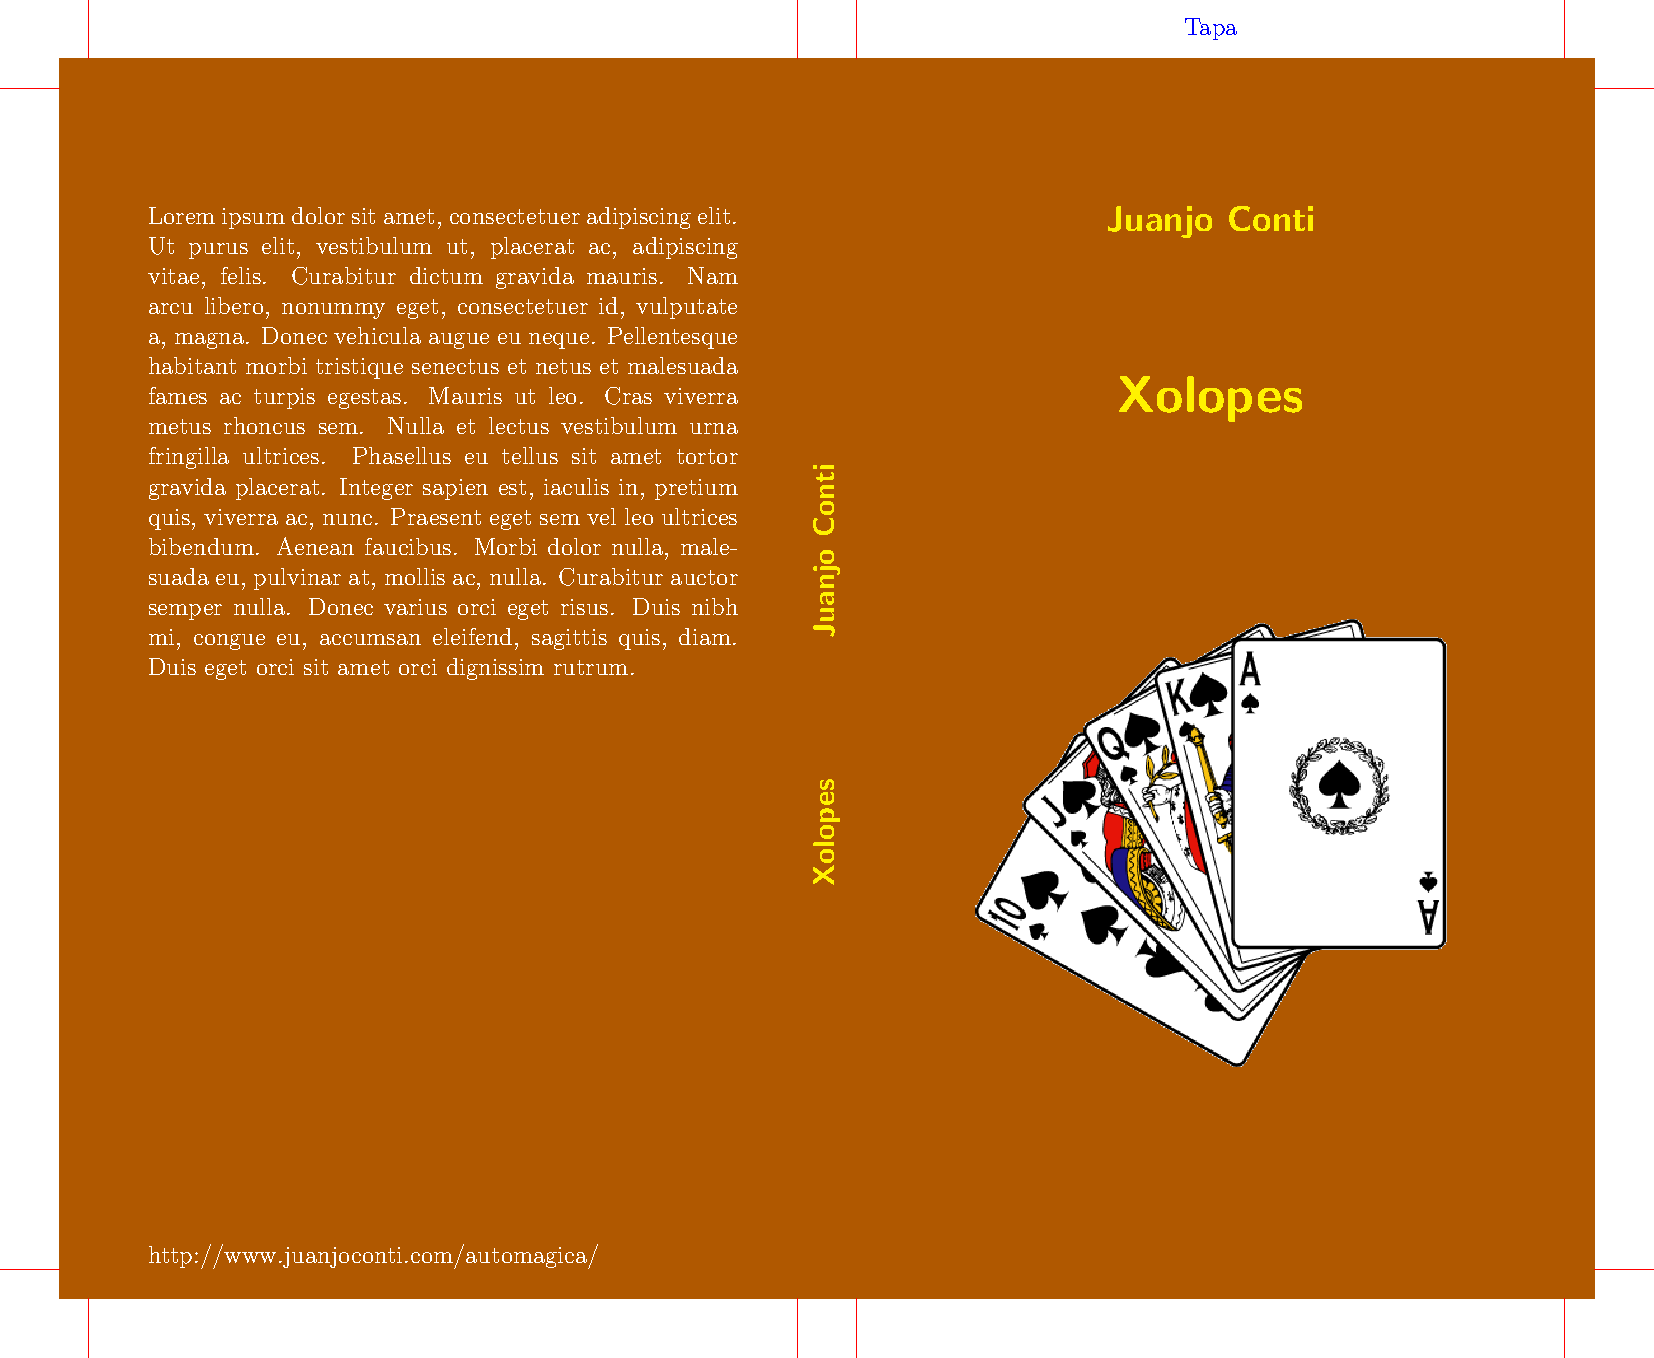
\includegraphics{figures/cover}
% \end{center}
% When we prepare a cover for printing, some marks are needed to know where to trim or fold the paper. These marks determine a special area of the sheet, which is called ``bleed'' (see the green area in the next figure). The background will be expanded onto the bleed, taking account of slight inaccuracy when trimming.
% \begin{center}
% \includegraphics{figures/coverscheme}
% \end{center}
% We get the following result after trimming:
% \begin{figure}[H]
% \centering
% \includegraphics{figures/result}
% \caption{}\label{fig:trimmed}
% \end{figure}
%
% \subsection{Book cover sizes}\label{subsec:sizes}
% We have to give the following sizes to prepare a cover (see the next figure): \texttt{coverwidth}, \texttt{coverheight}, \texttt{spinewidth}, \texttt{flapwidth}, \texttt{marklength}, \texttt{bleedwidth}.
% \begin{center}
% \includegraphics{figures/sizes}
% \end{center}
%
% \subsection{Loading class}
% The class \texttt{bookcover} requires the services of the class \texttt{article} and the following packages:
% \texttt{kvoptions}, \texttt{geometry}, \texttt{graphicx}, \texttt{calc}, \texttt{xcolor}, \texttt{ifthen}, \texttt{tikz}, \texttt{eso-pic}, \texttt{textpos}.
%
% \medskip\noindent
% Load the class as usual, with
% \begin{commandlst}
% \documentclass[!<options>!]{bookcover}
% \end{commandlst}
%
% \begin{center}
% \begin{tabular}{@{}llr@{}}
% \textbf{option}                        & \textbf{description}  & \textbf{default value}\\
% \hline
% \commandinline|coverwidth=!<length>!|  & See Subsection \ref{subsec:sizes}. & \texttt{170mm}\\
% \commandinline|coverheight=!<length>!| & See Subsection \ref{subsec:sizes}. & \texttt{240mm}\\
% \commandinline|spinewidth=!<length>!|  & See Subsection \ref{subsec:sizes}. &   \texttt{5mm}\\
% \commandinline|flapwidth=!<length>!|   & See Subsection \ref{subsec:sizes}. &   \texttt{0mm}\\
% \commandinline|marklength=!<length>!|  & See Subsection \ref{subsec:sizes}. &  \texttt{10mm}\\
% \commandinline|bleedwidth=!<length>!|  & See Subsection \ref{subsec:sizes}. &   \texttt{5mm}\\
% \commandinline|markthick=!<length>!|   & Thickness of marks.                & \texttt{0.4pt}\\
% \commandinline|markcolor=!<color>!|    & Color of marks.                    &   \texttt{red}\\
% \commandinline|10pt|                   & Normal font size is 10\,pt (default option).&\\
% \commandinline|11pt|                   & Normal font size is 11\,pt.&\\
% \commandinline|12pt|                   & Normal font size is 12\,pt.&\\
% \commandinline|grid|                   & Grid for checking sizes.&\\
% \commandinline|trimmed|                & It shows trimmed version (see Figure~\ref{fig:trimmed}).&\\
% \commandinline|bgtikznodes|            & For old method (see Subsubsection \ref{subsubsec:bgtikz}).&\\
% \commandinline|bgtikzclip|             & For old method (see Subsubsection \ref{subsubsec:bgtikz}).&\\
% \hline
% \end{tabular}
% \end{center}
%
% \bigskip\noindent\example
% \begin{examplelst}
% \documentclass[flapwidth=50mm,spinewidth=15mm]{bookcover}
% \end{examplelst}
%
% \section{Main method}\label{sec:mainmethod}
% \subsection{Commands}
% Use \commandinline{bookcover} environment to make a new book cover. In this environment, you can create a component of the book cover by the following command:
% \begin{commandlst}
% \bookcovercomponent{!<component type>!}{!<part>!}{!<content>!}
% \end{commandlst}
% \meta{component type} See Subsection \ref{subsec:componenttypes}.
%
% \medskip\noindent
% \meta{part} See Subsection \ref{subsec:parts-main-method} or \hyperref[appendix]{Appendix}.
%
% \medskip\noindent
% \meta{content} It depends on the \meta{component type} (see Subsection \ref{subsec:componenttypes}).
%
% \medskip\noindent
% Every |\bookcovercomponent| generates a layer on the sheet. The first one generates the bottom layer and the last one generates the top layer.
%
% \bigskip\noindent\example
% \begin{examplelst}
% \begin{bookcover}
%     \bookcovercomponent{color}{bg whole}{color=blue}
%     \bookcovercomponent{normal}{front}{
%         \vspace{5cm}
%         \begin{center}
%             \bfseries\huge Book title
%         \end{center}}
% \end{bookcover}
% \end{examplelst}
%
% \subsection{Parts in the main method}\label{subsec:parts-main-method}
% \subsubsection{Base background parts}
% \commandinline{bg back flap}, \commandinline{bg back}, \commandinline{bg spine}, \commandinline{bg front}, \commandinline{bg front flap}
%
%\medskip\noindent
% {\color{red}\faWarning} \emph{The background parts contain the bleed!}
%
% \paragraph{With flaps}
% \begin{center}
% \includegraphics{figures/bg1}
% \end{center}
% \paragraph{Without flaps}
% \begin{center}
% \includegraphics{figures/bg4}
% \end{center}
%
% \subsubsection{Base foreground parts}
% \commandinline{back flap}, \commandinline{back}, \commandinline{spine}, \commandinline{front}, \commandinline{front flap}, \commandinline{above back}, \commandinline{above front}, \commandinline{below back}, \commandinline{below front}
%
%\medskip\noindent
% {\color{red}\faWarning} \emph{The foreground parts don't contain the bleed!}
%
% \paragraph{With flaps}
% \begin{center}
% \includegraphics{figures/foreground1}
% \end{center}
% \paragraph{Without flaps}
% \begin{center}
% \includegraphics{figures/foreground2}
% \end{center}
%
% \subsubsection{Combined parts}
% The following combined parts are defined. You can see them in figures in the \hyperref[appendix]{Appendix}.
% \begin{center}
% \begin{tabular}{>{\color{command}\ttfamily}l@{\hspace{20mm}}>{\color{command}\ttfamily}l}
% bg back and flap            & back and flap\\
% bg back and spine           & back and spine\\
% bg front and spine          & front and spine\\
% bg front and flap           & front and flap\\
% bg back and flap and spine  & back and flap and spine\\
% bg front and flap and spine & front and flap and spine\\
% bg whole without front flap & whole without front flap\\
% bg whole without back flap  & whole without back flap\\
% bg whole without flaps      & whole without flaps\\
% bg whole                    & whole\\
% whole page                  &
% \end{tabular}
% \end{center}
%
% \subsection{Component types}\label{subsec:componenttypes}
% The following component types are defined: \commandinline{color}, \commandinline{picture}, \commandinline{tikz}, \commandinline{tikz clip}, \commandinline{normal}, \commandinline{center}, \commandinline{ruler}.
% \subsubsection[color]{Component type: \texttt{color}}
% \begin{commandlst}
% \bookcovercomponent{color}{!<part>!}{!<colors>!}
% \end{commandlst}
% \meta{colors} The options of the |\fill| in the \texttt{tikz} package:\\
% \indent\commandinline{color=!<color name>!} See \meta{color name} in the \texttt{xcolor} package.\\
% \indent\commandinline{top color=!<color name>!}\\
% \indent\commandinline{bottom color=!<color name>!}\\
% \indent\commandinline{middle color=!<color name>!}\\
% \indent\commandinline{inner color=!<color name>!}\\
% \indent\commandinline{outer color=!<color name>!}\\
% \indent\commandinline{ball color=!<color name>!}\\
% \indent\commandinline{shading angle=!<degree>!} It rotates the shading by the given angle.
%
% \bigskip\noindent\example
% \begin{examplelst}
% \begin{bookcover}
%     \bookcovercomponent{color}{bg whole without flaps}{
%         top color=white, bottom color=blue!50!black, shading angle=60}
% \end{bookcover}
% \end{examplelst}
%
% \subsubsection[picture]{Component type: \texttt{picture}}
% \begin{commandlst}
% \bookcovercomponent{picture}{!<part>!}{!<picture file>!}
% \end{commandlst}
% The picture will be rescaled according to the sizes of the \meta{part}.
%
% \bigskip\noindent\example
% \begin{examplelst}
% \begin{bookcover}
%     \bookcovercomponent{picture}{bg front flap}{fig.png}
% \end{bookcover}
% \end{examplelst}
%
% \subsubsection[tikz]{Component type: \texttt{tikz}}\label{subsubsec:tikz}
% \begin{commandlst}
% \bookcovercomponent{tikz}{!<part>!}{!<tikz code>!}
% \end{commandlst}
% The origin of the Ti\emph{k}Z figure is the lower left corner of the \meta{part}. Two rectangle nodes come into being: \commandinline{part} and \commandinline{trimmed part}. (Thank Zunbeltz Izaola for the idea.)
%
% \bigskip\noindent\example
% \begin{examplelst}
% \begin{bookcover}
% \bookcovercomponent{tikz}{bg whole}{
%     \fill[yellow] (part.south west) rectangle (part.north east);
%     \fill[gray] (trimmed part.south east) rectangle (trimmed part.north west);
%     \draw[green] (0,0) circle [radius=10mm];}
% \bookcovercomponent{tikz}{bg spine}{
%     \fill[orange] (part.center) circle [radius=8mm];}
% \end{bookcover}
% \end{examplelst}
% \begin{figure}[H]
% \centering
% \setlength{\fboxsep}{0pt}\setlength{\fboxrule}{.4pt}
% \fcolorbox{black!50}{white}{\includegraphics{figures/tikz}}
% \caption{}\label{fig:tikz}
% \end{figure}
%
% \subsubsection[tikz clip]{Component type: \texttt{tikz clip}}\label{subsubsec:tikz}
% \begin{commandlst}
% \bookcovercomponent{tikz clip}{!<part>!}{!<tikz code>!}
% \end{commandlst}
% It works the same as the \texttt{tikz} component type, but it clips the \meta{part}.
%
% \bigskip\noindent\example
% \begin{examplelst}
% \begin{bookcover}
% \bookcovercomponent{tikz clip}{bg whole}{
%     \fill[yellow] (part.south west) rectangle (part.north east);
%     \fill[gray] (trimmed part.south east) rectangle (trimmed part.north west);
%     \draw[green] (0,0) circle [radius=10mm];}
% \bookcovercomponent{tikz clip}{bg spine}{
%     \fill[orange] (part.center) circle [radius=8mm];}
% \end{bookcover}
% \end{examplelst}
% \begin{figure}[H]
% \centering
% \setlength{\fboxsep}{0pt}\setlength{\fboxrule}{.4pt}
% \fcolorbox{black!50}{white}{\includegraphics{figures/tikzclip}}
% \caption{}\label{fig:tikzclip}
% \end{figure}
%
% \subsubsection[normal]{Component type: \texttt{normal}}
% \begin{commandlst}
% \bookcovercomponent{normal}{!<part>!}{!<content>!}
% \end{commandlst}
% In this case, the \meta{content} is not specific. You can choose it as text or picture etc.
%
% \bigskip\noindent\example
% \begin{examplelst}
% \begin{bookcover}
%     \bookcovercomponent{normal}{front}{
%         \vspace{5cm}
%         \begin{center}
%             {\bfseries\huge Book title}\\[5mm]
%             \includegraphics[width=6cm]{fig.png}
%         \end{center}}
% \end{bookcover}
% \end{examplelst}
%
% \subsubsection[center]{Component type: \texttt{center}}
% \begin{commandlst}
% \bookcovercomponent{center}{!<part>!}{!<content>!}
% \end{commandlst}
% It works the same as the \texttt{normal} component type, but the position of the content is the center of the part (horizontally and vertically).
%
% \bigskip\noindent\example
% \begin{examplelst}
% \begin{bookcover}
%     \bookcovercomponent{center}{above front}{
%         \color{blue}Remark above front}
%     \bookcovercomponent{center}{spine}{
%         \rotatebox[origin=c]{90}{\bfseries\Large Book title}}
% \end{bookcover}
% \end{examplelst}
%
% \subsubsection[ruler]{Component type: \texttt{ruler}}
% Use the \texttt{ruler} component type to check the sizes of the part.
% \begin{commandlst}
% \bookcovercomponent{ruler}{!<part>!}{\setruler{!<coordsys>!}{!<shift x>!}{!<shift y>!}{!<color>!}}
% \end{commandlst}
% \meta{coordsys} The type of the coordinate system:\\
% \indent\commandinline{upper left } The origin is the upper left corner of the part.\\
% \indent\commandinline{upper right} The origin is the upper right corner of the part.\\
% \indent\commandinline{lower left } The origin is the lower left corner of the part.\\
% \indent\commandinline{lower right} The origin is the lower right corner of the part.
%
% \medskip\noindent
% \meta{shift x},\meta{shift y} Moving the origin of the ruler to the vector (\meta{shift x},\meta{shift y}).
%
% \medskip\noindent
% \meta{color} The color of the ruler.
%
% \bigskip\noindent\example
% \begin{examplelst}
% \begin{bookcover}
%    \bookcovercomponent{ruler}{back}{\setruler{upper left}{0cm}{0cm}{blue}}
%    \bookcovercomponent{ruler}{back}{\setruler{upper left}{2cm}{1cm}{black}}
%    \bookcovercomponent{ruler}{front}{\setruler{lower right}{0cm}{0cm}{green}}
%    \bookcovercomponent{ruler}{front}{\setruler{lower right}{2cm}{1cm}{gray}}
% \end{bookcover}
% \end{examplelst}
% \begin{figure}[H]
% \centering
% \setlength{\fboxsep}{0pt}\setlength{\fboxrule}{.4pt}
% \fcolorbox{black!50}{white}{\includegraphics{figures/ruler}}
% \end{figure}
%
% \subsection{Defining component type}
% New component types are defined using the command:
% \begin{commandlst}
% \newbookcovercomponenttype{!<new component type name>!}{!<formatting>!}
% \end{commandlst}
% Component types can be redefined using the command:
% \begin{commandlst}
% \renewbookcovercomponenttype{!<defined component type name>!}{!<formatting>!}
% \end{commandlst}
% Component types can be renamed using the command:
% \begin{commandlst}
% \newnamebookcovercomponenttype{!<new component type name>!}{!<defined component type name>!}
% \end{commandlst}
% You can use the following length commands in \meta{formatting}:
%
% \medskip\noindent
% \commandinline{\partwidth  } Width of the part.\\
% \commandinline{\partheight } Height of the part.
%
% \bigskip\noindent
% You have to referrence the content as \verb|#1|. 
%
% \bigskip\noindent\example
% \begin{examplelst}
% \documentclass[spinewidth=1cm]{bookcover}
% \newbookcovercomponenttype{center rotate}{
%     \parbox[t][\partheight][c]{\partwidth}{
%         \begin{center}
%             \rotatebox[origin=c]{90}{#1}
%         \end{center}}}
% \begin{document}
% \begin{bookcover}
%      \bookcovercomponent{center rotate}{spine}{Author -- Book title}
% \end{bookcover}
% \end{document}
% \end{examplelst}
%
% \subsection{Defining part}
% New parts are defined using the command:
% \begin{commandlst}
% \newbookcoverpart{!<new part name>!}{!<setting>!}
% \end{commandlst}
% Parts can be redefined using the command:
% \begin{commandlst}
% \renewbookcoverpart{!<defined part name>!}{!<setting>!}
% \end{commandlst}
% Parts can be renamed using the command:
% \begin{commandlst}
% \newnamebookcoverpart{!<new part name>!}{!<defined part name>!}
% \end{commandlst}
% In \meta{setting} you have to set the new part sizes, the coordinates of its upper left corner (the origin is the upper left corner of the printed box), and the parameters of the \texttt{trimmed part} rectangle node in \texttt{tikz} and \texttt{tikz clip} component types. For this purpose, use the following commands:
% \begin{commandlst}
% \setpartposx{!<coord x>!}
% \setpartposy{!<coord y>!}
% \setpartwidth{!<width>!}
% \setpartheight{!<height>!}
% \settrimmedpart{!<width minus>!}{!<height minus>!}{!<shift x>!}{!<shift y>!}
% \end{commandlst}
%
%\begin{center}
%\includegraphics{./figures/newpart}
%\end{center}
%
% \noindent To give the previous lengths, you can use the following length commands:
%
% \bigskip\noindent
% \commandinline{\marklength \bleedwidth \flapwidth \coverwidth \spinewidth \coverheight}
%
% \bigskip\noindent\example
% \begin{examplelst}
% \documentclass[flapwidth=3cm]{bookcover}
% \newbookcoverpart{bg half front}{
%     \setpartposx{\marklength+\bleedwidth+\flapwidth+\spinewidth+1.5\coverwidth}
%     \setpartposy{\marklength}
%     \setpartheight{\coverheight+2\bleedwidth}
%     \ifdim\flapwidth>0mm
%         \setpartwidth{.5\coverwidth}
%         \settrimmedpart{0pt}{2\bleedwidth}{0pt}{\bleedwidth}
%     \else
%         \setpartwidth{.5\coverwidth+\bleedwidth}
%         \settrimmedpart{\bleedwidth}{2\bleedwidth}{0pt}{\bleedwidth}\fi}
% \begin{document}
% \begin{bookcover}
% \bookcovercomponent{tikz}{bg half front}{
%     \fill[blue] (part.south west) rectangle (part.north east);
%     \fill[green] (trimmed part.south west) rectangle (trimmed part.north east);}
% \end{bookcover}
% \end{document}
% \end{examplelst}
%
% \subsection{Full examples}
% \subsubsection{A dust jacket}
% \begin{figure}[H]
% \centering
% \setlength{\fboxsep}{0pt}\setlength{\fboxrule}{.4pt}
% \fcolorbox{black!50}{white}{\includegraphics[width=\textwidth-.8pt]{example1}}
% \caption{}\label{fig:dustjacket}
% \end{figure}
% \lstinputlisting[style=examplefile]{example1.tex}
%
% \subsubsection{A two-sided book cover}
% \begin{figure}[H]
% \centering
% \setlength{\fboxsep}{0pt}\setlength{\fboxrule}{.4pt}
% \fcolorbox{black!50}{white}{\includegraphics[page=1,width=\textwidth-15mm]{example2}}
% \caption{Outside}\label{fig:twosidedbookcover-outside}
%
% \end{figure}
% \begin{figure}[H]
% \centering
% \setlength{\fboxsep}{0pt}\setlength{\fboxrule}{.4pt}
% \fcolorbox{black!50}{white}{\includegraphics[page=2,width=\textwidth-15mm]{example2}}
% \caption{Inside}\label{fig:twosidedbookcover-inside}
% \end{figure}
% \lstinputlisting[style=examplefile]{example2.tex}
%
% \subsubsection{Drawing bar code by pst-barcode package}
% \begin{figure}[H]
% \centering
% \setlength{\fboxsep}{0pt}\setlength{\fboxrule}{.4pt}
% \fcolorbox{black!50}{white}{\includegraphics[width=\textwidth-15mm]{figures/barcode}}
% \caption{}\label{fig:barcode}
% \end{figure}
%
% \begin{examplelst}
% \documentclass{bookcover}
% \usepackage{pst-barcode}
% \begin{document}
% \begin{bookcover} 
%     \bookcovercomponent{normal}{back}{
%         \vfill
%         \centering
%         \begin{pspicture}(1in,1.5in)
%             \psbarcode{1787-6117}{includetext height=1 width=1.5}{issn}
%         \end{pspicture}
%         \vspace{5mm}}
% \end{bookcover}
% \end{document}
% \end{examplelst}
%
% \noindent We can compile this file by \texttt{latex.exe} only. If you want to use another compiler, then choose the following way:
%
% \begin{examplelst}
% \documentclass{bookcover}
% 
% \usepackage{shellesc,filecontents}
% \begin{filecontents*}{bar.tex}
%     \documentclass{article}
%     \usepackage{pst-barcode}
%     \pagestyle{empty}
%     \begin{document}
%         \begin{pspicture}(1in,1.5in)
%             \psbarcode{1787-6117}{includetext height=1 width=1.5}{issn}
%         \end{pspicture}
%     \end{document}
% \end{filecontents*}
% 
% \ShellEscape{
%     latex bar.tex && 
%     dvips bar.dvi && 
%     ps2pdf bar.ps && 
%     pdfcrop -hires bar.pdf barcode.pdf}
% 
% \begin{document}
% \begin{bookcover}
%     \bookcovercomponent{normal}{back}{
%         \vfill
%         \centering
%         \includegraphics{barcode}
%         \vspace{5mm}}
% \end{bookcover}
% \end{document}
% \end{examplelst}
%
% \noindent The command to compile this file is the following:
% \begin{commandlinelst}
%      pdflatex -shell-escape filename
% \end{commandlinelst}
% or
% \begin{commandlinelst}
%      xelatex -shell-escape filename
% \end{commandlinelst}
% or
% \begin{commandlinelst}
%      lualatex -shell-escape filename
% \end{commandlinelst}
%
% \noindent where the \texttt{filename} is not \texttt{bar.tex} or \texttt{barcode.tex}. The following code works by \texttt{xelatex.exe} without option \texttt{-shell-escape}:
%
% \begin{examplelst}
% \documentclass{bookcover}
% \usepackage{pst-barcode}
% \begin{document}
% \makeatletter\TP@absposfalse\makeatother
% \newgeometry{left=0em,top=-1em}
% \begin{bookcover} 
%     \bookcovercomponent{normal}{back}{
%         \vfill
%         \centering
%         \begin{pspicture}(1in,1.5in)
%             \psbarcode{1787-6117}{includetext height=1 width=1.5}{issn}
%         \end{pspicture}
%         \vspace{5mm}}
% \end{bookcover}
% \end{document}
% \end{examplelst}
%
% \section{Old method}
% \begin{info}
% \color{red}\large\faWarning\ \textbf{Attention!} The goal of the \emph{old method} is to be compatible with the earlier versions of the \texttt{bookcover} class. It is recommended to use the \hyperref[sec:mainmethod]{\em main method} in the future, because it is much more flexible than the old one!
% \end{info}
%
% \subsection{Commands}
% \begin{commandlst}
% \setbookcover{!<main layer>!}{!<part>!}{!<content>!}
% \end{commandlst}
% \meta{main layer} See the following subsubsections.\\ 
% \indent\commandinline{bgcolor}, \commandinline{bgpic}, \commandinline{bgtikz}, \commandinline{fgfirst}, \commandinline{fgsecond}
%
% \medskip\noindent The \meta{part} and the \meta{content} depend on the \meta{main layer} (see the following subsubsections).
%
% \begin{commandlst}
% \makebookcover
% \end{commandlst}
%
% \subsubsection{Background colors}
% \begin{commandlst}
% \setbookcover{bgcolor}{!<background part>!}{!<colors>!}
% \end{commandlst}
% \meta{background part} See Subsubsection \ref{subsubsec:background}:\\ 
% \indent\commandinline{back}, \commandinline{front}, \commandinline{spine}, \commandinline{front flap}, \commandinline{back flap}, \commandinline{whole without flaps}, \commandinline{whole}
%
% \medskip\noindent 
% \meta{colors} The options of the |\fill| in the \texttt{tikz} package:\\
% \indent\commandinline{color=!<color name>!} See \meta{color name} in the \texttt{xcolor} package.\\ 
% \indent\commandinline{top color=!<color name>!}\\ 
% \indent\commandinline{bottom color=!<color name>!}\\ 
% \indent\commandinline{middle color=!<color name>!}\\ 
% \indent\commandinline{inner color=!<color name>!}\\ 
% \indent\commandinline{outer color=!<color name>!}\\ 
% \indent\commandinline{ball color=!<color name>!}\\ 
% \indent\commandinline{shading angle=!<degree>!} It rotates the shading by the given angle.
%
% \bigskip\noindent\example
% \begin{examplelst}
% \setbookcover{bgcolor}{whole without flaps}{
%     top color=white, bottom color=blue!50!black, shading angle=60}
% \end{examplelst}
%
% \subsubsection{Background pictures}
% \begin{commandlst}
% \setbookcover{bgpic}{!<background part>!}{!<picture file>!}
% \end{commandlst}
% \meta{background part} See Subsubsection \ref{subsubsec:background}:\\ 
% \indent\commandinline{back}, \commandinline{front}, \commandinline{spine}, \commandinline{front flap}, \commandinline{back flap}, \commandinline{whole without flaps}, \commandinline{whole}
%
% \medskip\noindent The picture will be rescaled according to the sizes of the current background part.
%
% \bigskip\noindent\example
% \begin{examplelst}
% \setbookcover{bgpic}{front flap}{fig.png}
% \end{examplelst}
%
% \subsubsection{Background Ti\emph{k}Z figures}\label{subsubsec:bgtikz}
% \begin{commandlst}
% \setbookcover{bgtikz}{!<background part>!}{!<tikz code>!}
% \end{commandlst}
% \meta{background part} See Subsubsection \ref{subsubsec:background}:\\ 
% \indent\commandinline{back}, \commandinline{front}, \commandinline{spine}, \commandinline{front flap}, \commandinline{back flap}, \commandinline{whole without flaps}, \commandinline{whole}
%
% \medskip\noindent
% The Ti\emph{k}Z figure will be placed to the upper left corner of the current background part, without resizing.
%
% \bigskip\noindent\example
% \begin{examplelst}
% \setbookcover{bgtikz}{back}{
%     \fill[blue] (0mm,250mm)--(100mm,250mm)--(100mm,245mm)--(0mm,110mm)--cycle;
%     \fill[yellow] (5mm,5mm)--(175mm,245mm)--(175mm,0mm)--(5mm,0mm)--cycle;}
% \end{examplelst}
%
% \medskip\noindent
% Using the option \texttt{bgtikznodes} of the document class:
%
% \medskip\noindent
% \begin{itemize}
% \item the origin moves to the lower left corner of the current background part;
% \item two rectangle nodes come into being: \commandinline{part} and \commandinline{trimmed part}.
% \end{itemize}
%
% \bigskip\noindent\example
% \begin{examplelst}
% \setbookcover{bgtikz}{whole}{
%     \fill[yellow] (part.south west) rectangle (part.north east);
%     \fill[gray] (trimmed part.south east) rectangle (trimmed part.north west);
%     \draw[green] (0,0) circle [radius=10mm];}
% \setbookcover{bgtikz}{spine}{
%     \fill[orange] (part.center) circle [radius=8mm];}
% \end{examplelst}
% \noindent See Figure~\ref{fig:tikz}. The option \texttt{bgtikzclip} of the document class works the same as \texttt{bgtikznodes}, but it clips the current part. For example, you can see the output of the previous code with option \texttt{bgtikzclip} in Figure~\ref{fig:tikzclip}.
%
% \subsubsection{First foreground}
% \begin{commandlst}
% \setbookcover{fgfirst}{!<foreground part>!}{!<content>!}
% \end{commandlst}
% \meta{foreground part} See Subsubsection \ref{subsubsec:foreground}:\\ 
% \indent\commandinline{back}, \commandinline{front}, \commandinline{spine}, \commandinline{front flap}, \commandinline{back flap}, \commandinline{above front}, \commandinline{below front}, \commandinline{above back}, \commandinline{below back}
%
% \medskip\noindent The first foreground is the top layer of the book cover (see Subsection \ref{subsec:layers}).
%
% \bigskip\noindent\example
% \begin{examplelst}
% \setbookcover{fgfirst}{spine}{
%     \vfill
%     \begin{center}
%         \rotatebox[origin=c]{90}{\bfseries Book title}
%     \end{center}
%     \vfill}
% \end{examplelst}
%
% \subsubsection{Second foreground}
% \begin{commandlst}
% \setbookcover{fgsecond}{!<foreground part>!}{!<content>!}
% \end{commandlst}
% \meta{foreground part} See Subsubsection \ref{subsubsec:foreground}:\\ 
% \indent\commandinline{back}, \commandinline{front}, \commandinline{spine}, \commandinline{front flap}, \commandinline{back flap}
%
% \medskip\noindent The second foreground is under the first foreground (see Subsection \ref{subsec:layers}).
%
% \bigskip\noindent\example
% \begin{examplelst}
% \setbookcover{fgsecond}{front}{
%     \vfill
%     \begin{center}
%         \includegraphics[width=80mm]{pic.png}
%     \end{center}
%     \vfill}
% \setbookcover{fgfirst}{front}{
%     \vfill
%     \begin{center}
%         TEXT
%     \end{center}
%     \vfill}
% \end{examplelst}
%
% \subsubsection{Making book cover}
% \commandinline{\makebookcover} 
%
% \medskip\noindent
% This command makes the book cover by using the contents of the background and foreground. 
%
% \subsection{Parts in the old method}
%
% \subsubsection{Background parts}\label{subsubsec:background}
% {\color{red}\faWarning} \emph{The background parts contain the bleed!}
%
% \paragraph{With flaps} 
% \begin{center}
% \includegraphics{figures/background1}\\[4mm]
% \includegraphics{figures/background2}\\[4mm]
% \includegraphics{figures/background3}
% \end{center}
% \paragraph{Without flaps} 
% \begin{center}
% \includegraphics{figures/background4}\\[4mm]
% \includegraphics{figures/background5}
% \end{center}
%
% \subsubsection{Foreground parts}\label{subsubsec:foreground}
% {\color{red}\faWarning} \emph{The foreground parts don't contain the bleed!}
%
% \paragraph{With flaps} 
% \begin{center}
% \includegraphics{figures/foreground1}
% \end{center}
% \paragraph{Without flaps} 
% \begin{center}
% \includegraphics{figures/foreground2}
% \end{center}
%
% \subsection{Layers}\label{subsec:layers}
% In the following table we can see the hierarchy of the layers:
%
% \bigskip
% \begin{center}
% \begin{tabular}{@{}ll@{}c@{}}
% \cline{1-2} 
%  \multirow{2}*{|fgfirst|}  & |above front|, |below front|, |above back|, |below back|& \color{layer}\emph{top layer}\\
%                            & |back|, |front|, |spine|, |front flap|, |back flap|     &\color{layer}$\uparrow$\\ 
% \cline{1-2}
% |fgsecond| & |back|, |front|, |spine|, |front flap|, |back flap|&\color{layer}$\uparrow$\\
% \cline{1-2}
% & |back|, |front|, |spine|, |front flap|, |back flap| &\color{layer}$\uparrow$\\
% |bgtikz| &  |whole without flaps| &\color{layer}$\uparrow$\\ 
% & |whole| &\color{layer}$\uparrow$\\
% \cline{1-2}
% & |back|, |front|, |spine|, |front flap|, |back flap| &\color{layer}$\uparrow$\\
% |bgpic| &  |whole without flaps| &\color{layer}$\uparrow$\\ 
% & |whole| &\color{layer}$\uparrow$\\
% \cline{1-2}
% & |back|, |front|, |spine|, |front flap|, |back flap| &\color{layer}$\uparrow$\\
% |bgcolor| &  |whole without flaps| &\color{layer}$\uparrow$\\ 
% & |whole| & \color{layer}\emph{bottom layer}\\
% \cline{1-2}
% \end{tabular} 
% \end{center}
% \bigskip\noindent For example, in case
% \begin{examplelst}
% \setbookcover{bgpic}{whole}{fig1.jpg}
% \setbookcover{bgpic}{front}{fig2.jpg}
% \setbookcover{fgsecond}{front}{fig3.jpg}
% \setbookcover{fgfirst}{front}{TEXT}
% \end{examplelst}
% \noindent the \texttt{TEXT} is above the \texttt{fig3.jpg}, the \texttt{fig3.jpg} is above the \texttt{fig2.jpg} and the \texttt{fig2.jpg} is above the \texttt{fig1.jpg}.
%
% \subsection{Full examples}
% \subsubsection{A dust jacket}
% See Figure \ref{fig:dustjacket}.
% \lstinputlisting[style=examplefile]{example1-oldmethod.tex}
%
% \subsubsection{A two-sided book cover}
% See Figure \ref{fig:twosidedbookcover-outside} and \ref{fig:twosidedbookcover-inside}.
% \lstinputlisting[style=examplefile]{example2-oldmethod.tex}
%
% \subsubsection{Drawing bar code by pst-barcode package}
%
% See Figure \ref{fig:barcode}.
%
% \begin{examplelst}
% \documentclass{bookcover}
% \usepackage{pst-barcode}
% \begin{document}
%     \setbookcover{fgfirst}{back}{
%         \vfill
%         \centering
%         \begin{pspicture}(1in,1.5in)
%             \psbarcode{1787-6117}{includetext height=1 width=1.5}{issn}
%         \end{pspicture}
%         \vspace{5mm}}
%     \makebookcover
% \end{document}
% \end{examplelst}
%
% \noindent We can compile this file by \texttt{latex.exe} only. If you want to use another compiler, then choose the following way:
%
% \begin{examplelst}
% \documentclass{bookcover}
% 
% \usepackage{shellesc,filecontents}
% \begin{filecontents*}{bar.tex}
%     \documentclass{article}
%     \usepackage{pst-barcode}
%     \pagestyle{empty}
%     \begin{document}
%         \begin{pspicture}(1in,1.5in)
%             \psbarcode{1787-6117}{includetext height=1 width=1.5}{issn}
%         \end{pspicture}
%     \end{document}
% \end{filecontents*}
% 
% \ShellEscape{
%     latex bar.tex && 
%     dvips bar.dvi && 
%     ps2pdf bar.ps && 
%     pdfcrop -hires bar.pdf barcode.pdf}
% 
% \begin{document}
%     \setbookcover{fgfirst}{back}{
%         \vfill
%         \centering
%         \includegraphics{barcode}
%         \vspace{5mm}}
%     \makebookcover
% \end{document}
% \end{examplelst}
%
% \noindent The command to compile this file is the following:
% \begin{commandlinelst}
%      pdflatex -shell-escape filename
% \end{commandlinelst}
% or
% \begin{commandlinelst}
%      xelatex -shell-escape filename
% \end{commandlinelst}
% or
% \begin{commandlinelst}
%      lualatex -shell-escape filename
% \end{commandlinelst}
%
% \noindent where the \texttt{filename} is not \texttt{bar.tex} or \texttt{barcode.tex}. The following code works by \texttt{xelatex.exe} without option \texttt{-shell-escape}:
%
% \begin{examplelst}
% \documentclass{bookcover}
% \usepackage{pst-barcode}
% \begin{document}
% \makeatletter\TP@absposfalse\makeatother
% \newgeometry{left=0em,top=-1em}
%     \setbookcover{fgfirst}{back}{
%         \vfill
%         \centering
%         \begin{pspicture}(1in,1.5in)
%             \psbarcode{1787-6117}{includetext height=1 width=1.5}{issn}
%         \end{pspicture}
%         \vspace{5mm}}
%     \makebookcover
% \end{document}
% \end{examplelst}
%
% \newpage
% \thispagestyle{empty}
% \vspace*{8cm}
% \section*{\centering\Huge Appendix}
% \addcontentsline{toc}{section}{Appendix}
%
% \includepdfset{nup=2x5,delta=4mm 4mm,noautoscale,frame}
% \includepdf[pages=1-10,pagecommand={\section*{\centering Background parts in the main method (width flaps)}\label{appendix}\addcontentsline{toc}{subsection}{Parts in the main method}}]{figures/parts.pdf}
% \includepdf[pages=11-16,pagecommand={\section*{\centering Background parts in the main method (width flaps)}}]{figures/parts.pdf}
% \includepdf[pages=17-26,pagecommand={\section*{\centering Foreground parts in the main method (width flaps)}}]{figures/parts.pdf}
% \includepdf[pages=27-35,pagecommand={\section*{\centering Foreground parts in the main method (width flaps)}}]{figures/parts.pdf}
% \includepdf[pages=36-42,pagecommand={\section*{\centering Background parts in the main method (widthout flaps)}}]{figures/parts.pdf}
% \includepdf[pages=43-52,pagecommand={\section*{\centering Foreground parts in the main method (widthout flaps)}}]{figures/parts.pdf}
%
% \StopEventually{}
%
% \section*{\centering Implementation}\addcontentsline{toc}{subsection}{Implementation}
% 
%    \begin{macrocode}
%%
%% OPTIONS
\RequirePackage{kvoptions}
\SetupKeyvalOptions{family=bookcover,prefix=bookcover@}
\DeclareVoidOption{10pt}{\PassOptionsToClass{10pt}{article}}
\DeclareVoidOption{11pt}{\PassOptionsToClass{11pt}{article}}
\DeclareVoidOption{12pt}{\PassOptionsToClass{12pt}{article}}
\DeclareVoidOption{grid}{\PassOptionsToPackage{grid}{eso-pic}}
\DeclareStringOption[170mm]{coverwidth}
\DeclareStringOption[240mm]{coverheight}
\DeclareStringOption[5mm]{spinewidth}
\DeclareStringOption[0mm]{flapwidth}
\DeclareStringOption[10mm]{marklength}
\DeclareStringOption[.4pt]{markthick}
\DeclareStringOption[5mm]{bleedwidth}
\DeclareStringOption[red]{markcolor}
\DeclareBoolOption[false]{trimmed}
\DeclareBoolOption[false]{bgtikznodes}% for old method
\DeclareBoolOption[false]{bgtikzclip}% for old method
\ProcessKeyvalOptions{bookcover}
\ifbookcover@bgtikzclip\bookcover@bgtikznodestrue\fi% for old method

%% CLASS AND PACKAGES
\LoadClass{article}
\RequirePackage{geometry,graphicx,calc,xcolor,ifthen,tikz,eso-pic}
\RequirePackage[absolute]{textpos}

%% PAGE STYLE
\pagestyle{empty}

%% NEW IF
\newif\if@inbookcoverenv

%% USER LENGTHS
\newlength{\coverwidth}
\newlength{\coverheight}
\newlength{\spinewidth}
\newlength{\flapwidth}
\newlength{\marklength}
\newlength{\markthick}
\newlength{\bleedwidth}

%% INTERNAL LENGTHS
\newlength{\bookcover@xpos@}
\newlength{\bookcover@ypos@}
\newlength{\bookcover@partwidth@}
\newlength{\bookcover@partheight@}
\newlength{\bookcover@tikz@trimmed@part@width@minus}
\newlength{\bookcover@tikz@trimmed@part@height@minus}
\newlength{\bookcover@tikz@trimmed@part@push@right}
\newlength{\bookcover@tikz@trimmed@part@push@up}
\newlength{\bookcover@ruler@xshift}
\newlength{\bookcover@ruler@yshift}
\let\partheight\bookcover@partheight@
\let\partwidth\bookcover@partwidth@

%% USER LENGTHS SETTING
\setlength{\coverwidth}{\bookcover@coverwidth}
\setlength{\coverheight}{\bookcover@coverheight}
\setlength{\spinewidth}{\bookcover@spinewidth}
\setlength{\flapwidth}{\bookcover@flapwidth}
\setlength{\marklength}{\bookcover@marklength}
\setlength{\markthick}{\bookcover@markthick}
\setlength{\bleedwidth}{\bookcover@bleedwidth}
\setlength{\paperwidth}{2\marklength+2\bleedwidth+2\coverwidth+2\flapwidth+\spinewidth}
\setlength{\paperheight}{2\marklength+2\bleedwidth+\coverheight}
\setlength{\parindent}{0pt}

%% INTERNAL LENGTHS SETTING
\def\bookcover@xpos#1{\setlength{\bookcover@xpos@}{#1}}
\def\bookcover@ypos#1{\setlength{\bookcover@ypos@}{#1}}
\def\bookcover@partwidth#1{\setlength{\bookcover@partwidth@}{#1}}
\def\bookcover@partheight#1{\setlength{\bookcover@partheight@}{#1}}
\def\bookcover@tikz@trimmed@part@param#1#2#3#4{%
    \setlength{\bookcover@tikz@trimmed@part@width@minus}{#1}%
    \setlength{\bookcover@tikz@trimmed@part@height@minus}{#2}
    \setlength{\bookcover@tikz@trimmed@part@push@right}{#3}
    \setlength{\bookcover@tikz@trimmed@part@push@up}{#4}}
\def\bookcover@bgtikz@trimmed@part@param#1#2{
    \bookcover@tikz@trimmed@part@param{#1}{2\bleedwidth}{#2}{\bleedwidth}}% for old method
\let\setpartposx\bookcover@xpos
\let\setpartposy\bookcover@ypos
\let\setpartwidth\bookcover@partwidth
\let\setpartheight\bookcover@partheight
\let\settrimmedpart\bookcover@tikz@trimmed@part@param

%% GRID
\ifESO@grid
    \setlength{\markthick}{2pt}
    \def\bookcover@markcolor{red}\fi

%% MARKS
\def\bookcover@vmark{
    \begin{textblock*}{\bookcover@partwidth@}(\bookcover@xpos@,\bookcover@ypos@)
        {\color{\bookcover@markcolor}\rule[0pt]{\markthick}{\marklength}}
    \end{textblock*}}

\def\bookcover@hmark{
    \begin{textblock*}{\bookcover@partwidth@}(\bookcover@xpos@,\bookcover@ypos@)
        {\color{\bookcover@markcolor}\rule[0pt]{\marklength}{\markthick}}
    \end{textblock*}}

\def\bookcover@marks{
    \bookcover@ypos{0mm}
    \bookcover@partwidth{\markthick}
    \bookcover@xpos{\marklength+\bleedwidth-.5\markthick}
    \bookcover@vmark
    \ifdim\flapwidth>0mm
        \bookcover@xpos{\marklength+\bleedwidth+\flapwidth-.5\markthick}
        \bookcover@vmark\fi
    \bookcover@xpos{\marklength+\bleedwidth+\flapwidth+\coverwidth-.5\markthick}
    \bookcover@vmark
    \bookcover@xpos{\marklength+\bleedwidth+\flapwidth+\coverwidth+\spinewidth-.5\markthick}
    \bookcover@vmark
    \ifdim\flapwidth>0mm
        \bookcover@xpos{\marklength+\bleedwidth+\flapwidth+2\coverwidth+\spinewidth-.5\markthick}
        \bookcover@vmark\fi
    \bookcover@xpos{\marklength+\bleedwidth+2\flapwidth+2\coverwidth+\spinewidth-.5\markthick}
    \bookcover@vmark
    \bookcover@ypos{\paperheight-\marklength}
    \bookcover@partwidth{\markthick}
    \bookcover@xpos{\marklength+\bleedwidth-.5\markthick}
    \bookcover@vmark
    \ifdim\flapwidth>0mm
        \bookcover@xpos{\marklength+\bleedwidth+\flapwidth-.5\markthick}
        \bookcover@vmark\fi
    \bookcover@xpos{\marklength+\bleedwidth+\flapwidth+\coverwidth-.5\markthick}
    \bookcover@vmark
    \bookcover@xpos{\marklength+\bleedwidth+\flapwidth+\coverwidth+\spinewidth-.5\markthick}
    \bookcover@vmark
    \ifdim\flapwidth>0mm
        \bookcover@xpos{\marklength+\bleedwidth+\flapwidth+2\coverwidth+\spinewidth-.5\markthick}
        \bookcover@vmark\fi
    \bookcover@xpos{\marklength+\bleedwidth+2\flapwidth+2\coverwidth+\spinewidth-.5\markthick}
    \bookcover@vmark
    \bookcover@xpos{0mm}
    \bookcover@partwidth{\marklength}
    \bookcover@ypos{\marklength+\bleedwidth-.5\markthick}
    \bookcover@hmark
    \bookcover@ypos{\marklength+\bleedwidth+\coverheight-.5\markthick}
    \bookcover@hmark
    \bookcover@xpos{\paperwidth-\marklength}
    \bookcover@partwidth{\marklength}
    \bookcover@ypos{\marklength+\bleedwidth-.5\markthick}
    \bookcover@hmark
    \bookcover@ypos{\marklength+\bleedwidth+\coverheight-.5\markthick}
    \bookcover@hmark}

%% TRIMMING
\def\bookcover@trimming{
    \begin{textblock*}{\paperwidth}(0mm,0mm)
        \begin{tikzpicture}
            \begin{scope}[color=white]
                \fill(0,0)--
                     (\paperwidth,0)--
                     (\paperwidth,\marklength+\bleedwidth)--
                     (0,\marklength+\bleedwidth)--cycle;
                \fill(0,\paperheight)--
                     (\paperwidth,\paperheight)--
                     (\paperwidth,\paperheight-\marklength-\bleedwidth)--
                     (0,\paperheight-\marklength-\bleedwidth)--cycle;
                \fill(0,0)--
                     (\marklength+\bleedwidth,0)--
                     (\marklength+\bleedwidth,\paperheight)--
                     (0,\paperheight)--cycle;
                \fill(\paperwidth-\marklength-\bleedwidth,0)--
                     (\paperwidth,0)--
                     (\paperwidth,\paperheight)--
                     (\paperwidth-\marklength-\bleedwidth,\paperheight)--cycle;
            \end{scope}
            \draw[color=\bookcover@markcolor,line width=\markthick]
                 (\marklength+\bleedwidth,\marklength+\bleedwidth)--
                 (\paperwidth-\marklength-\bleedwidth,\marklength+\bleedwidth)--
                 (\paperwidth-\marklength-\bleedwidth,\paperheight-\marklength-\bleedwidth)--
                 (\marklength+\bleedwidth,\paperheight-\marklength-\bleedwidth)--cycle;
        \end{tikzpicture}
    \end{textblock*}
    \bookcover@ypos{\bleedwidth}
    \bookcover@partwidth{\markthick}
    \ifdim\flapwidth>0mm
        \bookcover@xpos{\marklength+\bleedwidth+\flapwidth-.5\markthick}
        \bookcover@vmark
        \bookcover@xpos{\marklength+\bleedwidth+\flapwidth+2\coverwidth+\spinewidth-.5\markthick}
        \bookcover@vmark\fi
    \bookcover@xpos{\marklength+\bleedwidth+\flapwidth+\coverwidth-.5\markthick}
    \bookcover@vmark
    \bookcover@xpos{\marklength+\bleedwidth+\flapwidth+\coverwidth+\spinewidth-.5\markthick}
    \bookcover@vmark
    \bookcover@ypos{\paperheight-\marklength-\bleedwidth}
    \bookcover@partwidth{\markthick}
    \ifdim\flapwidth>0mm
        \bookcover@xpos{\marklength+\bleedwidth+\flapwidth-.5\markthick}
        \bookcover@vmark
        \bookcover@xpos{\marklength+\bleedwidth+\flapwidth+2\coverwidth+\spinewidth-.5\markthick}
        \bookcover@vmark\fi
    \bookcover@xpos{\marklength+\bleedwidth+\flapwidth+\coverwidth-.5\markthick}
    \bookcover@vmark
    \bookcover@xpos{\marklength+\bleedwidth+\flapwidth+\coverwidth+\spinewidth-.5\markthick}
    \bookcover@vmark}

%% BOOKCOVER COMPONENT
\long\def\bookcovercomponent#1#2#3{
    \if@inbookcoverenv\else
        \@latexerr{\string\bookcovercomponent\space is not in 'bookcover' environment.}{}\fi
    \bookcover@xpos{0pt}
    \bookcover@ypos{0pt}
    \bookcover@partwidth{0pt}
    \bookcover@partheight{0pt}
    \bookcover@tikz@trimmed@part@param{0pt}{0pt}{0pt}{0pt}
    \@ifundefined{bookcover@part@param@#2}{\@latexerr{Part '#2' undefined.}{}}{
        \@ifundefined{bookcover@componenttype@#1}{\@latexerr{Component type '#1' undefined.}{}}{
            \ifx#3\@empty\else
                \csname bookcover@part@param@#2\endcsname
                \ifdim\bookcover@partwidth@>0mm
                    \ifdim\bookcover@partheight@>0mm
                        \csname bookcover@componenttype@#1\endcsname{#3}\fi\fi\fi}}}

%% BOOKCOVER ENVIRONMENT
\def\bookcover{\@inbookcoverenvtrue}
\def\endbookcover{
    \bookcover@marks
    \ifbookcover@trimmed\bookcover@trimming\fi
    \mbox{}\newpage\@inbookcoverenvfalse}

%% NEW BOOKCOVER PART
\def\newbookcoverpart#1#2{
    \@ifundefined{bookcover@part@param@#1}{
        \expandafter\def\csname bookcover@part@param@#1\endcsname{#2}}
    {\@latexerr{Part '#1' already defined.}{}}}

%% RENEW BOOKCOVER PART
\def\renewbookcoverpart#1#2{
    \@ifundefined{bookcover@part@param@#1}{\@latexerr{Part '#1' undefined.}{}}{
        \expandafter\def\csname bookcover@part@param@#1\endcsname{#2}}}

%% NEW NAME BOOKCOVER PART
\def\newnamebookcoverpart#1#2{
    \@ifundefined{bookcover@part@param@#1}{
        \@ifundefined{bookcover@part@param@#2}{\@latexerr{Part '#2' undefined.}{}}{
            \expandafter\def\csname bookcover@part@param@#1\endcsname{%
                \csname bookcover@part@param@#2\endcsname}}}
    {\@latexerr{Part '#1' already defined.}{}}}

%% NEW BOOKCOVER COMPONENT TYPE
\def\newbookcovercomponenttype#1#2{
    \@ifundefined{bookcover@componenttype@#1}{
        \long\expandafter\def\csname bookcover@componenttype@#1\endcsname##1{
        \begin{textblock*}{\bookcover@partwidth@}(\bookcover@xpos@,\bookcover@ypos@)
        #2
        \end{textblock*}}}
    {\@latexerr{Component type '#1' already defined.}{}}}

%% RENEW BOOKCOVER COMPONENT TYPE
\def\renewbookcovercomponenttype#1#2{
    \@ifundefined{bookcover@componenttype@#1}{\@latex@error{Component type '#1' undefined.}{}}{
        \long\expandafter\def\csname bookcover@componenttype@#1\endcsname##1{
        \begin{textblock*}{\bookcover@partwidth@}(\bookcover@xpos@,\bookcover@ypos@)
        #2
        \end{textblock*}}}}

%% NEW NAME BOOKCOVER COMPONENT TYPE
\def\newnamebookcovercomponenttype#1#2{
    \@ifundefined{bookcover@componenttype@#1}{
        \@ifundefined{bookcover@componenttype@#2}{\@latexerr{Component type '#2' undefined.}{}}{
            \expandafter\def\csname bookcover@componenttype@#1\endcsname{%
                \csname bookcover@componenttype@#2\endcsname}}}
    {\@latexerr{Component type '#1' already defined.}{}}}

%% COMPONENT TYPES
\newbookcovercomponenttype{color}{
    \tikz\fill[#1] (0,0) rectangle (\bookcover@partwidth@,\bookcover@partheight@);}

\newbookcovercomponenttype{picture}{
    \includegraphics[width=\bookcover@partwidth@,height=\bookcover@partheight@]{#1}}

\newbookcovercomponenttype{tikz}{
    \begin{tikzpicture}[overlay,yshift=-\bookcover@partheight@]
    \begin{scope}[transparent,line width=0pt]
        \pgfset{minimum width=\bookcover@partwidth@,minimum height=\bookcover@partheight@}
        \pgfnode{rectangle}{south west}{}{part}{\pgfusepath{draw}}
        \pgfset{minimum width=\bookcover@partwidth@-\bookcover@tikz@trimmed@part@width@minus,
                minimum height=\bookcover@partheight@-\bookcover@tikz@trimmed@part@height@minus}
        \pgftransformshift{\pgfpoint{\bookcover@tikz@trimmed@part@push@right}
                                    {\bookcover@tikz@trimmed@part@push@up}}
        \pgfnode{rectangle}{south west}{}{trimmed part}{\pgfusepath{draw}}
    \end{scope}
    #1
    \end{tikzpicture}}

\newbookcovercomponenttype{tikz clip}{
    \begin{tikzpicture}[overlay,yshift=-\bookcover@partheight@]
    \begin{scope}[transparent,line width=0pt]
        \pgfset{minimum width=\bookcover@partwidth@,minimum height=\bookcover@partheight@}
        \pgfnode{rectangle}{south west}{}{part}{\pgfusepath{draw}}
        \pgfset{minimum width=\bookcover@partwidth@-\bookcover@tikz@trimmed@part@width@minus,
                minimum height=\bookcover@partheight@-\bookcover@tikz@trimmed@part@height@minus}
        \pgftransformshift{\pgfpoint{\bookcover@tikz@trimmed@part@push@right}
                                    {\bookcover@tikz@trimmed@part@push@up}}
        \pgfnode{rectangle}{south west}{}{trimmed part}{\pgfusepath{draw}}
    \end{scope}
    \clip (part.south west) rectangle (part.north east);
    #1
    \end{tikzpicture}}

\newbookcovercomponenttype{normal}{
    \parbox[t][\bookcover@partheight@][t]{\bookcover@partwidth@}{#1}}

\newbookcovercomponenttype{center}{
    \parbox[t][\bookcover@partheight@][c]{\bookcover@partwidth@}{\begin{center}#1\end{center}}}

\newbookcovercomponenttype{ruler}{
    \begin{tikzpicture}[overlay,x=1mm,y=1mm,inner sep=0pt,outer sep=3pt,yshift=-\bookcover@partheight@]
    #1
    \pgfmathsetmacro\xmax{round(.351459804*(\bookcover@partwidth@-\bookcover@ruler@xshift))}
    \pgfmathsetmacro\xnummax{round(.0351459804*(\bookcover@partwidth@-\bookcover@ruler@xshift))}
    \pgfmathsetmacro\ymax{round(.351459804*(\bookcover@partheight@-\bookcover@ruler@yshift))}
    \pgfmathsetmacro\ynummax{round(.0351459804*(\bookcover@partheight@-\bookcover@ruler@yshift))}
    \ifthenelse{\equal{\bookcover@ruler@coordsys}{lower left}}{
        \begin{scope}[xshift=\bookcover@ruler@xshift,yshift=\bookcover@ruler@yshift]
        \foreach \num in {0,1,...,\xmax}
        \draw (\num,0)--++(0,1);
        \foreach \num in {0,5,...,\xmax}
        \draw (\num,0)--++(0,1.5);
        \foreach \num in {0,10,...,\xmax}
        \draw (\num,0)--++(0,2);
        \foreach \num in {1,2,...,\xnummax}
        \node[anchor=south] at (10*\num,2)
            {\sffamily\scriptsize\num};
        \foreach \num in {0,1,...,\ymax}
        \draw (0,\num)--++(1,0);
        \foreach \num in {0,5,...,\ymax}
        \draw (0,\num)--++(1.5,0);
        \foreach \num in {0,10,...,\ymax}
        \draw (0,\num)--++(2,0);
        \foreach \num in {1,2,...,\ynummax}
        \node[anchor=west] at (2,10*\num)
            {\sffamily\scriptsize\num};
        \node[anchor=south] at (5,2)
            {\sffamily\scriptsize cm};
        \end{scope}}{}
    \ifthenelse{\equal{\bookcover@ruler@coordsys}{lower right}}{
        \begin{scope}[xshift=-\bookcover@ruler@xshift,yshift=\bookcover@ruler@yshift]
        \foreach \num in {0,1,...,\xmax}
        \draw (\bookcover@partwidth@-\num mm,0)--++(0,1);
        \foreach \num in {0,5,...,\xmax}
        \draw (\bookcover@partwidth@-\num mm,0)--++(0,1.5);
        \foreach \num in {0,10,...,\xmax}
        \draw (\bookcover@partwidth@-\num mm,0)--++(0,2);
        \foreach \num in {1,2,...,\xnummax}
        \node[anchor=south] at (\bookcover@partwidth@-10*\num mm,2)
            {\sffamily\scriptsize\num};
        \foreach \num in {0,1,...,\ymax}
        \draw (\bookcover@partwidth@,\num)--++(-1,0);
        \foreach \num in {0,5,...,\ymax}
        \draw (\bookcover@partwidth@,\num)--++(-1.5,0);
        \foreach \num in {0,10,...,\ymax}
        \draw (\bookcover@partwidth@,\num)--++(-2,0);
        \foreach \num in {1,2,...,\ynummax}
        \node[anchor=east] at (\bookcover@partwidth@-2mm,10*\num)
            {\sffamily\scriptsize\num};
        \node[anchor=south] at (\bookcover@partwidth@-5mm,2)
            {\sffamily\scriptsize cm};
        \end{scope}}{}
    \ifthenelse{\equal{\bookcover@ruler@coordsys}{upper left}}{
        \begin{scope}[xshift=\bookcover@ruler@xshift,yshift=-\bookcover@ruler@yshift]
        \foreach \num in {0,1,...,\xmax}
        \draw (\num,\bookcover@partheight@)--++(0,-1);
        \foreach \num in {0,5,...,\xmax}
        \draw (\num,\bookcover@partheight@)--++(0,-1.5);
        \foreach \num in {0,10,...,\xmax}
        \draw (\num,\bookcover@partheight@)--++(0,-2);
        \foreach \num in {1,2,...,\xnummax}
        \node[anchor=north] at (10*\num,\bookcover@partheight@-2mm)
            {\sffamily\scriptsize\num};
        \foreach \num in {0,1,...,\ymax}
        \draw (0,\bookcover@partheight@-\num mm)--++(1,0);
        \foreach \num in {0,5,...,\ymax}
        \draw (0,\bookcover@partheight@-\num mm)--++(1.5,0);
        \foreach \num in {0,10,...,\ymax}
        \draw (0,\bookcover@partheight@-\num mm)--++(2,0);
        \foreach \num in {1,2,...,\ynummax}
        \node[anchor=west] at (2,\bookcover@partheight@-10*\num mm)
            {\sffamily\scriptsize\num};
        \node[anchor=north] at (5,\bookcover@partheight@-2mm)
            {\sffamily\scriptsize\vphantom{1}cm};
        \end{scope}}{}
    \ifthenelse{\equal{\bookcover@ruler@coordsys}{upper right}}{
        \begin{scope}[xshift=-\bookcover@ruler@xshift,yshift=-\bookcover@ruler@yshift]
        \foreach \num in {0,1,...,\xmax}
        \draw (\bookcover@partwidth@-\num mm,\bookcover@partheight@)--++(0,-1);
        \foreach \num in {0,5,...,\xmax}
        \draw (\bookcover@partwidth@-\num mm,\bookcover@partheight@)--++(0,-1.5);
        \foreach \num in {0,10,...,\xmax}
        \draw (\bookcover@partwidth@-\num mm,\bookcover@partheight@)--++(0,-2);
        \foreach \num in {1,2,...,\xnummax}
        \node[anchor=north] at (\bookcover@partwidth@-10*\num mm,\bookcover@partheight@-2mm)
            {\sffamily\scriptsize\num};
        \foreach \num in {0,1,...,\ymax}
        \draw (\bookcover@partwidth@,\bookcover@partheight@-\num mm)--++(-1,0);
        \foreach \num in {0,5,...,\ymax}
        \draw (\bookcover@partwidth@,\bookcover@partheight@-\num mm)--++(-1.5,0);
        \foreach \num in {0,10,...,\ymax}
        \draw (\bookcover@partwidth@,\bookcover@partheight@-\num mm)--++(-2,0);
        \foreach \num in {1,2,...,\ynummax}
        \node[anchor=east] at (\bookcover@partwidth@-2mm,\bookcover@partheight@-10*\num mm)
            {\sffamily\scriptsize\num};
        \node[anchor=north] at (\bookcover@partwidth@-5mm,\bookcover@partheight@-2mm)
            {\sffamily\scriptsize\vphantom{1}cm};
        \end{scope}}{}
    \end{tikzpicture}}
\def\setruler#1#2#3#4{
    \def\bookcover@ruler@coordsys{#1}
    \setlength{\bookcover@ruler@xshift}{#2}
    \setlength{\bookcover@ruler@yshift}{#3}
    \color{#4}}

%% BOOKCOVER PARTS
\newbookcoverpart{bg back flap}{
    \ifdim\flapwidth>0mm
        \bookcover@ypos{\marklength}
        \bookcover@partheight{\coverheight+2\bleedwidth}
        \bookcover@xpos{\marklength}
        \bookcover@partwidth{\flapwidth+\bleedwidth}
        \bookcover@tikz@trimmed@part@param{\bleedwidth}{2\bleedwidth}{\bleedwidth}{\bleedwidth}\fi}

\newbookcoverpart{bg back}{
    \bookcover@ypos{\marklength}
    \bookcover@partheight{\coverheight+2\bleedwidth}
    \ifdim\flapwidth>0mm
        \bookcover@xpos{\marklength+\bleedwidth+\flapwidth}
        \bookcover@partwidth{\coverwidth}
        \bookcover@tikz@trimmed@part@param{0pt}{2\bleedwidth}{0pt}{\bleedwidth}
    \else
        \bookcover@xpos{\marklength}
        \bookcover@partwidth{\coverwidth+\bleedwidth}
        \bookcover@tikz@trimmed@part@param{\bleedwidth}{2\bleedwidth}{\bleedwidth}{\bleedwidth}\fi}

\newbookcoverpart{bg spine}{
    \bookcover@ypos{\marklength}
    \bookcover@partheight{\coverheight+2\bleedwidth}
    \bookcover@xpos{\marklength+\bleedwidth+\flapwidth+\coverwidth}
    \bookcover@partwidth{\spinewidth}
    \bookcover@tikz@trimmed@part@param{0pt}{2\bleedwidth}{0pt}{\bleedwidth}}

\newbookcoverpart{bg front}{
    \bookcover@ypos{\marklength}
    \bookcover@partheight{\coverheight+2\bleedwidth}
    \bookcover@xpos{\marklength+\bleedwidth+\flapwidth+\coverwidth+\spinewidth}
    \ifdim\flapwidth>0mm
        \bookcover@partwidth{\coverwidth}
        \bookcover@tikz@trimmed@part@param{0pt}{2\bleedwidth}{0pt}{\bleedwidth}
    \else
        \bookcover@partwidth{\coverwidth+\bleedwidth}
        \bookcover@tikz@trimmed@part@param{\bleedwidth}{2\bleedwidth}{0pt}{\bleedwidth}\fi}

\newbookcoverpart{bg front flap}{
    \ifdim\flapwidth>0mm
        \bookcover@ypos{\marklength}
        \bookcover@partheight{\coverheight+2\bleedwidth}
        \bookcover@xpos{\marklength+\bleedwidth+\flapwidth+2\coverwidth+\spinewidth}
        \bookcover@partwidth{\flapwidth+\bleedwidth}
        \bookcover@tikz@trimmed@part@param{\bleedwidth}{2\bleedwidth}{0pt}{\bleedwidth}\fi}

\newbookcoverpart{bg back and flap}{
    \bookcover@ypos{\marklength}
    \bookcover@partheight{\coverheight+2\bleedwidth}
    \bookcover@xpos{\marklength}
    \bookcover@partwidth{\bleedwidth+\flapwidth+\coverwidth}
    \bookcover@tikz@trimmed@part@param{\bleedwidth}{2\bleedwidth}{\bleedwidth}{\bleedwidth}}

\newbookcoverpart{bg back and spine}{
    \bookcover@ypos{\marklength}
    \bookcover@partheight{\coverheight+2\bleedwidth}
    \ifdim\flapwidth>0mm
        \bookcover@xpos{\marklength+\bleedwidth+\flapwidth}
        \bookcover@partwidth{\coverwidth+\spinewidth}
        \bookcover@tikz@trimmed@part@param{0pt}{2\bleedwidth}{0pt}{\bleedwidth}
    \else
        \bookcover@xpos{\marklength}
        \bookcover@partwidth{\coverwidth+\bleedwidth+\spinewidth}
        \bookcover@tikz@trimmed@part@param{\bleedwidth}{2\bleedwidth}{\bleedwidth}{\bleedwidth}\fi}

\newbookcoverpart{bg front and spine}{
    \bookcover@ypos{\marklength}
    \bookcover@partheight{\coverheight+2\bleedwidth}
    \bookcover@xpos{\marklength+\bleedwidth+\flapwidth+\coverwidth}
    \ifdim\flapwidth>0mm
        \bookcover@partwidth{\coverwidth+\spinewidth}
        \bookcover@tikz@trimmed@part@param{0pt}{2\bleedwidth}{0pt}{\bleedwidth}
    \else
        \bookcover@partwidth{\coverwidth+\spinewidth+\bleedwidth}
        \bookcover@tikz@trimmed@part@param{\bleedwidth}{2\bleedwidth}{0pt}{\bleedwidth}\fi}

\newbookcoverpart{bg front and flap}{
    \bookcover@ypos{\marklength}
    \bookcover@partheight{\coverheight+2\bleedwidth}
    \bookcover@xpos{\marklength+\bleedwidth+\flapwidth+\coverwidth+\spinewidth}
    \bookcover@partwidth{\coverwidth+\flapwidth+\bleedwidth}
    \bookcover@tikz@trimmed@part@param{\bleedwidth}{2\bleedwidth}{0pt}{\bleedwidth}}

\newbookcoverpart{bg back and flap and spine}{
    \bookcover@ypos{\marklength}
    \bookcover@partheight{\coverheight+2\bleedwidth}
    \bookcover@xpos{\marklength}
    \bookcover@partwidth{\bleedwidth+\flapwidth+\coverwidth+\spinewidth}
    \bookcover@tikz@trimmed@part@param{\bleedwidth}{2\bleedwidth}{\bleedwidth}{\bleedwidth}}

\newbookcoverpart{bg whole without flaps}{
    \bookcover@ypos{\marklength}
    \bookcover@partheight{\coverheight+2\bleedwidth}
    \ifdim\flapwidth>0mm
        \bookcover@xpos{\marklength+\bleedwidth+\flapwidth}
        \bookcover@partwidth{2\coverwidth+\spinewidth}
        \bookcover@tikz@trimmed@part@param{0pt}{2\bleedwidth}{0pt}{\bleedwidth}
    \else
        \bookcover@xpos{\marklength}
        \bookcover@partwidth{2\coverwidth+2\bleedwidth+\spinewidth}
        \bookcover@tikz@trimmed@part@param{2\bleedwidth}{2\bleedwidth}{\bleedwidth}{\bleedwidth}\fi}

\newbookcoverpart{bg front and flap and spine}{
    \bookcover@ypos{\marklength}
    \bookcover@partheight{\coverheight+2\bleedwidth}
    \bookcover@xpos{\marklength+\bleedwidth+\flapwidth+\coverwidth}
    \bookcover@partwidth{\coverwidth+\flapwidth+\bleedwidth+\spinewidth}
    \bookcover@tikz@trimmed@part@param{\bleedwidth}{2\bleedwidth}{0pt}{\bleedwidth}}

\newbookcoverpart{bg whole without front flap}{
    \bookcover@ypos{\marklength}
    \bookcover@partheight{\coverheight+2\bleedwidth}
    \bookcover@xpos{\marklength}
    \ifdim\flapwidth>0mm
        \bookcover@partwidth{2\coverwidth+\flapwidth+\bleedwidth+\spinewidth}
        \bookcover@tikz@trimmed@part@param{\bleedwidth}{2\bleedwidth}{\bleedwidth}{\bleedwidth}
    \else
        \bookcover@partwidth{2\coverwidth+2\bleedwidth+\spinewidth}
        \bookcover@tikz@trimmed@part@param{2\bleedwidth}{2\bleedwidth}{\bleedwidth}{\bleedwidth}\fi}

\newbookcoverpart{bg whole without back flap}{
    \bookcover@ypos{\marklength}
    \bookcover@partheight{\coverheight+2\bleedwidth}
    \ifdim\flapwidth>0mm
        \bookcover@xpos{\marklength+\bleedwidth+\flapwidth}
        \bookcover@partwidth{2\coverwidth+\flapwidth+\bleedwidth+\spinewidth}
        \bookcover@tikz@trimmed@part@param{\bleedwidth}{2\bleedwidth}{0mm}{\bleedwidth}
    \else
        \bookcover@xpos{\marklength}
        \bookcover@partwidth{2\coverwidth+2\bleedwidth+\spinewidth}
        \bookcover@tikz@trimmed@part@param{2\bleedwidth}{2\bleedwidth}{\bleedwidth}{\bleedwidth}\fi}

\newbookcoverpart{bg whole}{
    \bookcover@ypos{\marklength}
    \bookcover@partheight{\coverheight+2\bleedwidth}
    \bookcover@xpos{\marklength}
    \bookcover@partwidth{2\coverwidth+2\bleedwidth+2\flapwidth+\spinewidth}
    \bookcover@tikz@trimmed@part@param{2\bleedwidth}{2\bleedwidth}{\bleedwidth}{\bleedwidth}}

\newbookcoverpart{whole page}{
    \bookcover@partheight{\paperheight}
    \bookcover@partwidth{\paperwidth}}

\newbookcoverpart{back flap}{
    \ifdim\flapwidth>0mm
        \bookcover@ypos{\marklength+\bleedwidth}
        \bookcover@partheight{\coverheight}
        \bookcover@xpos{\marklength+\bleedwidth}
        \bookcover@partwidth{\flapwidth}\fi}

\newbookcoverpart{back}{
    \bookcover@ypos{\marklength+\bleedwidth}
    \bookcover@partheight{\coverheight}
    \bookcover@xpos{\marklength+\bleedwidth+\flapwidth}
    \bookcover@partwidth{\coverwidth}}

\newbookcoverpart{spine}{
    \bookcover@ypos{\marklength+\bleedwidth}
    \bookcover@partheight{\coverheight}
    \bookcover@xpos{\marklength+\bleedwidth+\flapwidth+\coverwidth}
    \bookcover@partwidth{\spinewidth}}

\newbookcoverpart{front}{
    \bookcover@ypos{\marklength+\bleedwidth}
    \bookcover@partheight{\coverheight}
    \bookcover@xpos{\marklength+\bleedwidth+\flapwidth+\coverwidth+\spinewidth}
    \bookcover@partwidth{\coverwidth}}

\newbookcoverpart{front flap}{
    \ifdim\flapwidth>0mm
        \bookcover@ypos{\marklength+\bleedwidth}
        \bookcover@partheight{\coverheight}
        \bookcover@xpos{\marklength+\bleedwidth+\flapwidth+2\coverwidth+\spinewidth}
        \bookcover@partwidth{\flapwidth}\fi}

\newbookcoverpart{above front}{
    \ifdim\marklength>0mm
        \bookcover@xpos{\marklength+\bleedwidth+\flapwidth+\coverwidth+\spinewidth}
        \bookcover@ypos{0mm}
        \bookcover@partwidth{\coverwidth}
        \bookcover@partheight{\marklength}\fi}

\newbookcoverpart{below front}{
    \ifdim\marklength>0mm
        \bookcover@xpos{\marklength+\bleedwidth+\flapwidth+\coverwidth+\spinewidth}
        \bookcover@ypos{\marklength+2\bleedwidth+\coverheight}
        \bookcover@partwidth{\coverwidth}
        \bookcover@partheight{\marklength}\fi}

\newbookcoverpart{above back}{
    \ifdim\marklength>0mm
        \bookcover@xpos{\marklength+\bleedwidth+\flapwidth}
        \bookcover@ypos{0mm}
        \bookcover@partwidth{\coverwidth}
        \bookcover@partheight{\marklength}\fi}

\newbookcoverpart{below back}{
    \ifdim\marklength>0mm
        \bookcover@xpos{\marklength+\bleedwidth+\flapwidth}
        \bookcover@ypos{\marklength+2\bleedwidth+\coverheight}
        \bookcover@partwidth{\coverwidth}
        \bookcover@partheight{\marklength}\fi}

\newbookcoverpart{back and flap}{
    \bookcover@ypos{\marklength+\bleedwidth}
    \bookcover@xpos{\marklength+\bleedwidth}
    \bookcover@partwidth{\flapwidth+\coverwidth}
    \bookcover@partheight{\coverheight}}

\newbookcoverpart{back and spine}{
    \bookcover@ypos{\marklength+\bleedwidth}
    \bookcover@partheight{\coverheight}
    \bookcover@xpos{\marklength+\bleedwidth+\flapwidth}
    \bookcover@partwidth{\coverwidth+\spinewidth}}

\newbookcoverpart{front and spine}{
    \bookcover@ypos{\marklength+\bleedwidth}
    \bookcover@partheight{\coverheight}
    \bookcover@xpos{\marklength+\bleedwidth+\flapwidth+\coverwidth}
    \bookcover@partwidth{\coverwidth+\spinewidth}}

\newbookcoverpart{front and flap}{
    \bookcover@ypos{\marklength+\bleedwidth}
    \bookcover@partheight{\coverheight}
    \bookcover@xpos{\marklength+\bleedwidth+\flapwidth+\coverwidth+\spinewidth}
    \bookcover@partwidth{\coverwidth+\flapwidth}}

\newbookcoverpart{back and flap and spine}{
    \bookcover@ypos{\marklength+\bleedwidth}
    \bookcover@xpos{\marklength+\bleedwidth}
    \bookcover@partwidth{\flapwidth+\coverwidth+\spinewidth}
    \bookcover@partheight{\coverheight}}

\newbookcoverpart{whole without flaps}{
    \bookcover@ypos{\marklength+\bleedwidth}
    \bookcover@partheight{\coverheight}
    \bookcover@xpos{\marklength+\bleedwidth+\flapwidth}
    \bookcover@partwidth{2\coverwidth+\spinewidth}}

\newbookcoverpart{front and flap and spine}{
    \bookcover@ypos{\marklength+\bleedwidth}
    \bookcover@partheight{\coverheight}
    \bookcover@xpos{\marklength+\bleedwidth+\flapwidth+\coverwidth}
    \bookcover@partwidth{\coverwidth+\flapwidth+\spinewidth}}

\newbookcoverpart{whole without front flap}{
    \bookcover@ypos{\marklength+\bleedwidth}
    \bookcover@partheight{\coverheight}
    \bookcover@xpos{\marklength+\bleedwidth}
    \bookcover@partwidth{2\coverwidth+\flapwidth+\spinewidth}}

\newbookcoverpart{whole without back flap}{
    \bookcover@ypos{\marklength+\bleedwidth}
    \bookcover@partheight{\coverheight}
    \bookcover@xpos{\marklength+\bleedwidth+\flapwidth}
    \bookcover@partwidth{2\coverwidth+\flapwidth+\spinewidth}}

\newbookcoverpart{whole}{
    \bookcover@ypos{\marklength+\bleedwidth}
    \bookcover@partheight{\coverheight}
    \bookcover@xpos{\marklength+\bleedwidth}
    \bookcover@partwidth{2\coverwidth+2\flapwidth+\spinewidth}}

%%%%%%%%%%%%%%%%
%% OLD METHOD %%
%%%%%%%%%%%%%%%%

%% MAIN LAYERS
\def\bookcover@bgcolor#1{
    \begin{textblock*}{\bookcover@partwidth@}(\bookcover@xpos@,\bookcover@ypos@)
        \tikz\fill\expandafter[#1] (0,0) rectangle (\bookcover@partwidth@,\bookcover@partheight@);
    \end{textblock*}}

\def\bookcover@bgpic#1{
    \begin{textblock*}{\bookcover@partwidth@}(\bookcover@xpos@,\bookcover@ypos@)
        \includegraphics[width=\bookcover@partwidth@,height=\bookcover@partheight@]{#1}
    \end{textblock*}}

\def\bookcover@bgtikz#1{
    \begin{textblock*}{\bookcover@partwidth@}(\bookcover@xpos@,\bookcover@ypos@)
     \ifbookcover@bgtikznodes
        \begin{tikzpicture}[overlay,yshift=-\bookcover@partheight@]
        \begin{scope}[transparent,line width=0pt]
            \pgfset{minimum width=\bookcover@partwidth@,minimum height=\bookcover@partheight@}
            \pgfnode{rectangle}{south west}{}{current part}{\pgfusepath{draw}}% for v1.1.1
            \pgfnode{rectangle}{south west}{}{part}{\pgfusepath{draw}}
            \pgfset{minimum width=\bookcover@partwidth@-\bookcover@tikz@trimmed@part@width@minus,
                    minimum height=\bookcover@partheight@-\bookcover@tikz@trimmed@part@height@minus}
            \pgftransformshift{\pgfpoint{\bookcover@tikz@trimmed@part@push@right}
                                        {\bookcover@tikz@trimmed@part@push@up}}
            \pgfnode{rectangle}{south west}{}{current trimmed part}{\pgfusepath{draw}}% for v1.1.1
            \pgfnode{rectangle}{south west}{}{trimmed part}{\pgfusepath{draw}}
        \end{scope}
        \ifbookcover@bgtikzclip
            \clip (part.south west) rectangle (part.north east);\fi
    \else\begin{tikzpicture}\fi
        #1
        \end{tikzpicture}
    \end{textblock*}}

\def\bookcover@fg#1{
    \begin{textblock*}{\bookcover@partwidth@}(\bookcover@xpos@,\bookcover@ypos@)
        \parbox[t][\bookcover@partheight@][t]{\bookcover@partwidth@}{#1}
    \end{textblock*}}

\def\bookcover@remark#1{
    \begin{textblock*}{\bookcover@partwidth@}(\bookcover@xpos@,\bookcover@ypos@)
        \parbox[t][\bookcover@partheight@][c]{\bookcover@partwidth@}{\begin{center}#1\end{center}}
    \end{textblock*}}

%% RESET DATAS
\def\bookcover@reset{
    \def\bookcover@bgcolor@whole{}
    \def\bookcover@bgcolor@wholewf{}
    \def\bookcover@bgcolor@back{}
    \def\bookcover@bgcolor@front{}
    \def\bookcover@bgcolor@backflap{}
    \def\bookcover@bgcolor@frontflap{}
    \def\bookcover@bgcolor@spine{}
    \def\bookcover@bgpic@whole{}
    \def\bookcover@bgpic@wholewf{}
    \def\bookcover@bgpic@back{}
    \def\bookcover@bgpic@front{}
    \def\bookcover@bgpic@backflap{}
    \def\bookcover@bgpic@frontflap{}
    \def\bookcover@bgpic@spine{}
    \def\bookcover@bgtikz@whole{}
    \def\bookcover@bgtikz@wholewf{}
    \def\bookcover@bgtikz@back{}
    \def\bookcover@bgtikz@front{}
    \def\bookcover@bgtikz@backflap{}
    \def\bookcover@bgtikz@frontflap{}
    \def\bookcover@bgtikz@spine{}
    \def\bookcover@fgfirst@back{}
    \def\bookcover@fgfirst@front{}
    \def\bookcover@fgfirst@spine{}
    \def\bookcover@fgfirst@backflap{}
    \def\bookcover@fgfirst@frontflap{}
    \def\bookcover@fgfirst@abovefront{}
    \def\bookcover@fgfirst@belowfront{}
    \def\bookcover@fgfirst@aboveback{}
    \def\bookcover@fgfirst@belowback{}
    \def\bookcover@fgsecond@back{}
    \def\bookcover@fgsecond@front{}
    \def\bookcover@fgsecond@spine{}
    \def\bookcover@fgsecond@backflap{}
    \def\bookcover@fgsecond@frontflap{}}
\bookcover@reset

%% SET BOOKCOVER
\long\def\setbookcover#1#2#3{
    \ifthenelse{\equal{#1}{bgcolor}}{
        \ifthenelse{\equal{#2}{whole}}{\def\bookcover@bgcolor@whole{#3}}{}
        \ifthenelse{\equal{#2}{whole without flaps}}{\def\bookcover@bgcolor@wholewf{#3}}{}
        \ifthenelse{\equal{#2}{back}}{\def\bookcover@bgcolor@back{#3}}{}
        \ifthenelse{\equal{#2}{front}}{\def\bookcover@bgcolor@front{#3}}{}
        \ifthenelse{\equal{#2}{back flap}}{\def\bookcover@bgcolor@backflap{#3}}{}
        \ifthenelse{\equal{#2}{front flap}}{\def\bookcover@bgcolor@frontflap{#3}}{}
        \ifthenelse{\equal{#2}{spine}}{\def\bookcover@bgcolor@spine{#3}}{}}{}
    \ifthenelse{\equal{#1}{bgpic}}{
        \ifthenelse{\equal{#2}{whole}}{\def\bookcover@bgpic@whole{#3}}{}
        \ifthenelse{\equal{#2}{whole without flaps}}{\def\bookcover@bgpic@wholewf{#3}}{}
        \ifthenelse{\equal{#2}{back}}{\def\bookcover@bgpic@back{#3}}{}
        \ifthenelse{\equal{#2}{front}}{\def\bookcover@bgpic@front{#3}}{}
        \ifthenelse{\equal{#2}{back flap}}{\def\bookcover@bgpic@backflap{#3}}{}
        \ifthenelse{\equal{#2}{front flap}}{\def\bookcover@bgpic@frontflap{#3}}{}
        \ifthenelse{\equal{#2}{spine}}{\def\bookcover@bgpic@spine{#3}}{}}{}
    \ifthenelse{\equal{#1}{bgtikz}}{
        \ifthenelse{\equal{#2}{whole}}{\def\bookcover@bgtikz@whole{#3}}{}
        \ifthenelse{\equal{#2}{whole without flaps}}{\def\bookcover@bgtikz@wholewf{#3}}{}
        \ifthenelse{\equal{#2}{back}}{\def\bookcover@bgtikz@back{#3}}{}
        \ifthenelse{\equal{#2}{front}}{\def\bookcover@bgtikz@front{#3}}{}
        \ifthenelse{\equal{#2}{back flap}}{\def\bookcover@bgtikz@backflap{#3}}{}
        \ifthenelse{\equal{#2}{front flap}}{\def\bookcover@bgtikz@frontflap{#3}}{}
        \ifthenelse{\equal{#2}{spine}}{\def\bookcover@bgtikz@spine{#3}}{}}{}
    \ifthenelse{\equal{#1}{fgfirst}}{
        \ifthenelse{\equal{#2}{back}}{\def\bookcover@fgfirst@back{#3}}{}
        \ifthenelse{\equal{#2}{front}}{\def\bookcover@fgfirst@front{#3}}{}
        \ifthenelse{\equal{#2}{spine}}{\def\bookcover@fgfirst@spine{#3}}{}
        \ifthenelse{\equal{#2}{back flap}}{\def\bookcover@fgfirst@backflap{#3}}{}
        \ifthenelse{\equal{#2}{front flap}}{\def\bookcover@fgfirst@frontflap{#3}}{}
        \ifthenelse{\equal{#2}{remark}}{\def\bookcover@fgfirst@abovefront{#3}}{}% for v1.0
        \ifthenelse{\equal{#2}{above front}}{\def\bookcover@fgfirst@abovefront{#3}}{}
        \ifthenelse{\equal{#2}{below front}}{\def\bookcover@fgfirst@belowfront{#3}}{}
        \ifthenelse{\equal{#2}{above back}}{\def\bookcover@fgfirst@aboveback{#3}}{}
        \ifthenelse{\equal{#2}{below back}}{\def\bookcover@fgfirst@belowback{#3}}{}}{}
    \ifthenelse{\equal{#1}{fgsecond}}{
        \ifthenelse{\equal{#2}{back}}{\def\bookcover@fgsecond@back{#3}}{}
        \ifthenelse{\equal{#2}{front}}{\def\bookcover@fgsecond@front{#3}}{}
        \ifthenelse{\equal{#2}{spine}}{\def\bookcover@fgsecond@spine{#3}}{}
        \ifthenelse{\equal{#2}{back flap}}{\def\bookcover@fgsecond@backflap{#3}}{}
        \ifthenelse{\equal{#2}{front flap}}{\def\bookcover@fgsecond@frontflap{#3}}{}}{}}

%% MAKE BOOKCOVER
\def\makebookcover{
%% background parameters
\bookcover@ypos{\marklength}
\bookcover@partheight{\coverheight+2\bleedwidth}
%% {bgcolor}{whole}
\ifx\bookcover@bgcolor@whole\@empty\else
    \bookcover@xpos{\marklength}
    \bookcover@partwidth{2\coverwidth+2\bleedwidth+2\flapwidth+\spinewidth}
    \bookcover@bgcolor{\bookcover@bgcolor@whole}\fi
%% {bgcolor}{whole without flaps}
\ifx\bookcover@bgcolor@wholewf\@empty\else
    \ifdim\flapwidth>0mm
        \bookcover@xpos{\marklength+\bleedwidth+\flapwidth}
        \bookcover@partwidth{2\coverwidth+\spinewidth}
    \else
        \bookcover@xpos{\marklength}
        \bookcover@partwidth{2\coverwidth+2\bleedwidth+\spinewidth}\fi
    \bookcover@bgcolor{\bookcover@bgcolor@wholewf}\fi
%% {bgcolor}{back flap}
\ifx\bookcover@bgcolor@backflap\@empty\else\ifdim\flapwidth>0mm
    \bookcover@xpos{\marklength}
    \bookcover@partwidth{\flapwidth+\bleedwidth}
    \bookcover@bgcolor{\bookcover@bgcolor@backflap}\fi\fi
%% {bgcolor}{back}
\ifx\bookcover@bgcolor@back\@empty\else
    \ifdim\flapwidth>0mm
        \bookcover@xpos{\marklength+\bleedwidth+\flapwidth}
        \bookcover@partwidth{\coverwidth}
    \else
        \bookcover@xpos{\marklength}
        \bookcover@partwidth{\coverwidth+\bleedwidth}\fi
    \bookcover@bgcolor{\bookcover@bgcolor@back}\fi
%% {bgcolor}{spine}
\ifx\bookcover@bgcolor@spine\@empty\else
    \bookcover@xpos{\marklength+\bleedwidth+\flapwidth+\coverwidth}
    \bookcover@partwidth{\spinewidth}
    \bookcover@bgcolor{\bookcover@bgcolor@spine}\fi
%% {bgcolor}{front}
\ifx\bookcover@bgcolor@front\@empty\else
    \ifdim\flapwidth>0mm
        \bookcover@xpos{\marklength+\bleedwidth+\flapwidth+\coverwidth+\spinewidth}
        \bookcover@partwidth{\coverwidth}
    \else
        \bookcover@xpos{\marklength+\bleedwidth+\coverwidth+\spinewidth}
        \bookcover@partwidth{\coverwidth+\bleedwidth}\fi
    \bookcover@bgcolor{\bookcover@bgcolor@front}\fi
%% {bgcolor}{front flap}
\ifx\bookcover@bgcolor@frontflap\@empty\else\ifdim\flapwidth>0mm
    \bookcover@xpos{\marklength+\bleedwidth+\flapwidth+2\coverwidth+\spinewidth}
    \bookcover@partwidth{\flapwidth+\bleedwidth}
    \bookcover@bgcolor{\bookcover@bgcolor@frontflap}\fi\fi
%% {bgpic}{whole}
\ifx\bookcover@bgpic@whole\@empty\else
    \bookcover@xpos{\marklength}
    \bookcover@partwidth{2\coverwidth+2\bleedwidth+2\flapwidth+\spinewidth}
    \bookcover@bgpic{\bookcover@bgpic@whole}\fi
%% {bgpic}{whole without flaps}
\ifx\bookcover@bgpic@wholewf\@empty\else
    \ifdim\flapwidth>0mm
        \bookcover@xpos{\marklength+\bleedwidth+\flapwidth}
        \bookcover@partwidth{2\coverwidth+\spinewidth}
    \else
        \bookcover@xpos{\marklength}
        \bookcover@partwidth{2\coverwidth+2\bleedwidth+\spinewidth}\fi
    \bookcover@bgpic{\bookcover@bgpic@wholewf}\fi
%% {bgpic}{back flap}
\ifx\bookcover@bgpic@backflap\@empty\else\ifdim\flapwidth>0mm
    \bookcover@xpos{\marklength}
    \bookcover@partwidth{\flapwidth+\bleedwidth}
    \bookcover@bgpic{\bookcover@bgpic@backflap}\fi\fi
%% {bgpic}{back}
\ifx\bookcover@bgpic@back\@empty\else
    \ifdim\flapwidth>0mm
        \bookcover@xpos{\marklength+\bleedwidth+\flapwidth}
        \bookcover@partwidth{\coverwidth}
    \else
        \bookcover@xpos{\marklength}
        \bookcover@partwidth{\coverwidth+\bleedwidth}\fi
    \bookcover@bgpic{\bookcover@bgpic@back}\fi
%% {bgpic}{spine}
\ifx\bookcover@bgpic@spine\@empty\else
    \bookcover@xpos{\marklength+\bleedwidth+\flapwidth+\coverwidth}
    \bookcover@partwidth{\spinewidth}
    \bookcover@bgpic{\bookcover@bgpic@spine}\fi
%% {bgpic}{front}
\ifx\bookcover@bgpic@front\@empty\else
    \ifdim\flapwidth>0mm
        \bookcover@xpos{\marklength+\bleedwidth+\flapwidth+\coverwidth+\spinewidth}
        \bookcover@partwidth{\coverwidth}
    \else
        \bookcover@xpos{\marklength+\bleedwidth+\coverwidth+\spinewidth}
        \bookcover@partwidth{\coverwidth+\bleedwidth}\fi
    \bookcover@bgpic{\bookcover@bgpic@front}\fi
%% {bgpic}{front flap}
\ifx\bookcover@bgpic@frontflap\@empty\else\ifdim\flapwidth>0mm
    \bookcover@xpos{\marklength+\bleedwidth+\flapwidth+2\coverwidth+\spinewidth}
    \bookcover@partwidth{\flapwidth+\bleedwidth}
    \bookcover@bgpic{\bookcover@bgpic@frontflap}\fi\fi
%% {bgtikz}{whole}
\ifx\bookcover@bgtikz@whole\@empty\else
    \bookcover@xpos{\marklength}
    \bookcover@partwidth{2\coverwidth+2\bleedwidth+2\flapwidth+\spinewidth}
    \bookcover@bgtikz@trimmed@part@param{2\bleedwidth}{\bleedwidth}
    \bookcover@bgtikz{\bookcover@bgtikz@whole}\fi
%% {bgtikz}{whole without flaps}
\ifx\bookcover@bgtikz@wholewf\@empty\else
    \ifdim\flapwidth>0mm
        \bookcover@xpos{\marklength+\bleedwidth+\flapwidth}
        \bookcover@partwidth{2\coverwidth+\spinewidth}
        \bookcover@bgtikz@trimmed@part@param{0pt}{0pt}
    \else
        \bookcover@xpos{\marklength}
        \bookcover@partwidth{2\coverwidth+2\bleedwidth+\spinewidth}
        \bookcover@bgtikz@trimmed@part@param{2\bleedwidth}{\bleedwidth}\fi
    \bookcover@bgtikz{\bookcover@bgtikz@wholewf}\fi
%% {bgtikz}{back flap}
\ifx\bookcover@bgtikz@backflap\@empty\else\ifdim\flapwidth>0mm
    \bookcover@xpos{\marklength}
    \bookcover@partwidth{\flapwidth+\bleedwidth}
    \bookcover@bgtikz@trimmed@part@param{\bleedwidth}{\bleedwidth}
    \bookcover@bgtikz{\bookcover@bgtikz@backflap}\fi\fi
%% {bgtikz}{back}
\ifx\bookcover@bgtikz@back\@empty\else
    \ifdim\flapwidth>0mm
        \bookcover@xpos{\marklength+\bleedwidth+\flapwidth}
        \bookcover@partwidth{\coverwidth}
        \bookcover@bgtikz@trimmed@part@param{0pt}{0pt}
    \else
        \bookcover@xpos{\marklength}
        \bookcover@partwidth{\coverwidth+\bleedwidth}
        \bookcover@bgtikz@trimmed@part@param{\bleedwidth}{\bleedwidth}\fi
    \bookcover@bgtikz{\bookcover@bgtikz@back}\fi
%% {bgtikz}{spine}
\ifx\bookcover@bgtikz@spine\@empty\else
    \bookcover@xpos{\marklength+\bleedwidth+\flapwidth+\coverwidth}
    \bookcover@partwidth{\spinewidth}
    \bookcover@bgtikz@trimmed@part@param{0pt}{0pt}
    \bookcover@bgtikz{\bookcover@bgtikz@spine}\fi
%% {bgtikz}{front}
\ifx\bookcover@bgtikz@front\@empty\else
    \ifdim\flapwidth>0mm
        \bookcover@xpos{\marklength+\bleedwidth+\flapwidth+\coverwidth+\spinewidth}
        \bookcover@partwidth{\coverwidth}
        \bookcover@bgtikz@trimmed@part@param{0pt}{0pt}
    \else
        \bookcover@xpos{\marklength+\bleedwidth+\coverwidth+\spinewidth}
        \bookcover@partwidth{\coverwidth+\bleedwidth}
        \bookcover@bgtikz@trimmed@part@param{\bleedwidth}{0pt}\fi
    \bookcover@bgtikz{\bookcover@bgtikz@front}\fi
%% {bgtikz}{front flap}
\ifx\bookcover@bgtikz@frontflap\@empty\else\ifdim\flapwidth>0mm
    \bookcover@xpos{\marklength+\bleedwidth+\flapwidth+2\coverwidth+\spinewidth}
    \bookcover@partwidth{\flapwidth+\bleedwidth}
    \bookcover@bgtikz@trimmed@part@param{\bleedwidth}{0pt}
    \bookcover@bgtikz{\bookcover@bgtikz@frontflap}\fi\fi
%% foreground parameters
\bookcover@ypos{\marklength+\bleedwidth}
\bookcover@partheight{\coverheight}
%% {fgsecond}{back flap}
\ifx\bookcover@fgsecond@backflap\@empty\else\ifdim\flapwidth>0mm
    \bookcover@xpos{\marklength+\bleedwidth}
    \bookcover@partwidth{\flapwidth}
    \bookcover@fg{\bookcover@fgsecond@backflap}\fi\fi
%% {fgsecond}{back}
\ifx\bookcover@fgsecond@back\@empty\else
    \bookcover@xpos{\marklength+\bleedwidth+\flapwidth}
    \bookcover@partwidth{\coverwidth}
    \bookcover@fg{\bookcover@fgsecond@back}\fi
%% {fgsecond}{spine}
\ifx\bookcover@fgsecond@spine\@empty\else
    \bookcover@xpos{\marklength+\bleedwidth+\flapwidth+\coverwidth}
    \bookcover@partwidth{\spinewidth}
    \bookcover@fg{\bookcover@fgsecond@spine}\fi
%% {fgsecond}{front}
\ifx\bookcover@fgsecond@front\@empty\else
    \bookcover@xpos{\marklength+\bleedwidth+\flapwidth+\coverwidth+\spinewidth}
    \bookcover@partwidth{\coverwidth}
    \bookcover@fg{\bookcover@fgsecond@front}\fi
%% {fgsecond}{front flap}
\ifx\bookcover@fgsecond@frontflap\@empty\else\ifdim\flapwidth>0mm
    \bookcover@xpos{\marklength+\bleedwidth+\flapwidth+2\coverwidth+\spinewidth}
    \bookcover@partwidth{\flapwidth}
    \bookcover@fg{\bookcover@fgsecond@frontflap}\fi\fi
%% {fgfirst}{back flap}
\ifx\bookcover@fgfirst@backflap\@empty\else\ifdim\flapwidth>0mm
    \bookcover@xpos{\marklength+\bleedwidth}
    \bookcover@partwidth{\flapwidth}
    \bookcover@fg{\bookcover@fgfirst@backflap}\fi\fi
%% {fgfirst}{back}
\ifx\bookcover@fgfirst@back\@empty\else
    \bookcover@xpos{\marklength+\bleedwidth+\flapwidth}
    \bookcover@partwidth{\coverwidth}
    \bookcover@fg{\bookcover@fgfirst@back}\fi
%% {fgfirst}{spine}
\ifx\bookcover@fgfirst@spine\@empty\else
    \bookcover@xpos{\marklength+\bleedwidth+\flapwidth+\coverwidth}
    \bookcover@partwidth{\spinewidth}
    \bookcover@fg{\bookcover@fgfirst@spine}\fi
%% {fgfirst}{front}
\ifx\bookcover@fgfirst@front\@empty\else
    \bookcover@xpos{\marklength+\bleedwidth+\flapwidth+\coverwidth+\spinewidth}
    \bookcover@partwidth{\coverwidth}
    \bookcover@fg{\bookcover@fgfirst@front}\fi
%% {fgfirst}{front flap}
\ifx\bookcover@fgfirst@frontflap\@empty\else\ifdim\flapwidth>0mm
    \bookcover@xpos{\marklength+\bleedwidth+\flapwidth+2\coverwidth+\spinewidth}
    \bookcover@partwidth{\flapwidth}
    \bookcover@fg{\bookcover@fgfirst@frontflap}\fi\fi
%% {fgfirst}{above front} = {fgfirst}{remark} in v1.0
\ifx\bookcover@fgfirst@abovefront\@empty\else\ifdim\marklength>0mm
    \bookcover@xpos{\marklength+\bleedwidth+\flapwidth+\coverwidth+\spinewidth}
    \bookcover@ypos{0mm}
    \bookcover@partwidth{\coverwidth}
    \bookcover@partheight{\marklength}
    \bookcover@remark{\bookcover@fgfirst@abovefront}\fi\fi
%% {fgfirst}{below front}
\ifx\bookcover@fgfirst@belowfront\@empty\else\ifdim\marklength>0mm
    \bookcover@xpos{\marklength+\bleedwidth+\flapwidth+\coverwidth+\spinewidth}
    \bookcover@ypos{\marklength+2\bleedwidth+\coverheight}
    \bookcover@partwidth{\coverwidth}
    \bookcover@partheight{\marklength}
    \bookcover@remark{\bookcover@fgfirst@belowfront}\fi\fi
%% {fgfirst}{above back}
\ifx\bookcover@fgfirst@aboveback\@empty\else\ifdim\marklength>0mm
    \bookcover@xpos{\marklength+\bleedwidth+\flapwidth}
    \bookcover@ypos{0mm}
    \bookcover@partwidth{\coverwidth}
    \bookcover@partheight{\marklength}
    \bookcover@remark{\bookcover@fgfirst@aboveback}\fi\fi
%% {fgfirst}{below back}
\ifx\bookcover@fgfirst@belowback\@empty\else\ifdim\marklength>0mm
    \bookcover@xpos{\marklength+\bleedwidth+\flapwidth}
    \bookcover@ypos{\marklength+2\bleedwidth+\coverheight}
    \bookcover@partwidth{\coverwidth}
    \bookcover@partheight{\marklength}
    \bookcover@remark{\bookcover@fgfirst@belowback}\fi\fi
%% marks
\bookcover@marks
%% trimming
\ifbookcover@trimmed\bookcover@trimming\fi
%% new book cover
\mbox{}\newpage\bookcover@reset}
%    \end{macrocode}
% \Finale
\endinput